\PassOptionsToPackage{hyphens}{url}
\documentclass[fleqn,10pt]{article}
\usepackage[utf8]{inputenc}
\usepackage[T1]{fontenc}
\usepackage{amsmath,amssymb,amsfonts}
\usepackage{amsthm}
\newtheorem{theorem}{Theorem}
\newtheorem{proposition}{Proposition}
\newtheorem{lemma}{Lemma}
\newtheorem{corollary}{Corollary}
\newtheorem{remark}{Remark}
\newtheorem{definition}{Definition}
\usepackage{graphicx}
\graphicspath{{figures/}}
\usepackage{booktabs}
\usepackage{tabularx}
\usepackage{multirow}
\usepackage{hyperref}
\usepackage{xurl}
\usepackage{cite}
\usepackage{bm}
\usepackage{color}
\usepackage{lmodern}
\usepackage{authblk}
\usepackage{geometry}
\geometry{a4paper, margin=0.75in}
\usepackage{caption}
\usepackage{subcaption}

\hypersetup{
	colorlinks=true,
	linkcolor=blue,
	citecolor=blue,
	urlcolor=blue
}

\title{\textbf{Extending Multibody Simulation: Closed-Form Dynamics from URDF Models for Model-Based Control and Trajectory Optimization of Serial Manipulators}}

\author[1,2]{Ahmed Askar}

\affil[1]{Department of Mechatronics and Robotics Engineering, School of Innovative Design Engineering, Egypt-Japan University of Science and Technology (E-JUST), New Borg El-Arab City, Alexandria, Egypt}
\affil[2]{Department of Production Engineering and Mechanical Design, Faculty of Engineering, Mansoura University, Mansoura, Egypt}

\date{\today}

\begin{document}
	
	\maketitle
	
	\begin{abstract}
		Articulated robotics requires a dependable bridge between raw Unified Robot Description Format (URDF) descriptions and analytical, closed-form equations of motion. While physics simulators evaluate dynamics numerically, model-based control synthesis, trajectory optimization, and parameter identification require differentiable, algebraically inspectable mass, Coriolis, and gravitational representations. However, deriving white-box Lagrangian equations directly from unconstrained CAD-based URDFs faces three major obstacles: kinematic gauge ambiguities across joint coordinate frames, physically corrupted CAD inertia tensors, and severe symbolic expression explosion during Coriolis tensor expansion. In this work, we present an open, Denavit--Hartenberg (DH)-consistent URDF-to-analytical-dynamics pipeline featuring automated gauge resolution, physical realizability projection onto the rigid-body inertia cone, and derivation-phase algorithmic differentiation (AD) graph compression. We show that evaluating the Coriolis and centrifugal bias vector directly via an Euler--Lagrange generalized momentum directional derivative bounds the bias evaluation cost to a constant multiple of the mass-matrix cost: $\operatorname{cost}(\mathbf{c}_{\text{bias}}) \le (c_f + c_r) \cdot \operatorname{cost}(\bm{M}(\bm{q}))$. Across a systematic benchmark of serial manipulators spanning $n \in [3, 14]$ degrees of freedom, Common Subexpression Elimination (CSE) yields empirical scaling exponents of $\mathcal{O}(n^{2.29 \pm 0.08})$ for the momentum bias vector versus $\mathcal{O}(n^{3.25 \pm 0.12})$ for classical Christoffel expansions, reducing forward dynamics instruction opcodes by up to $75.5\%$ and accelerating single-step evaluation by up to $4.48\times$ ($1,419.7~\mu$s $\to 374.2~\mu$s at $n=14$). In an NLP sensitivity benchmark on 6-DOF and 7-DOF manipulators, this derivation-phase graph compression reduces Karush--Kuhn--Tucker (KKT) constraint Jacobian opcodes by up to $48.2\%$, cutting mean solve latency from $9.20$~s to $4.82$~s on redundant architectures under IPOPT ($1.91\times$ speedup) and mitigating active obstacle latency spikes by $45.7\%$. Validated across multi-vendor industrial manipulators with an autonomous fail-fast verification dashboard, our open-source framework ensures internal static algebraic consistency to double-precision machine epsilon ($<10^{-12}$~N$\cdot$m) and achieves sub-$100~\mu$s bare-metal dynamics throughput ($>10$~kHz), bridging the gap between descriptive robot models and certified analytical mechanics.
	\end{abstract}
	
%==============================================================================
\section*{Introduction}
%==============================================================================

Analytical formulations based on minimal kinematic parameterizations, most notably the standard Denavit--Hartenberg (DH) convention \cite{denavit1955kinematic, craig2005introduction, spong2020robot, siciliano2010robotics}, together with closed-form Euler--Lagrange dynamics, form the foundation of robot mechanics, nonlinear control, and robotics education. Such formulations explicitly reveal how kinematic geometry and inertial properties shape system behavior, enabling dynamics analysis, stability assessment, and systematic controller synthesis. Modern robotics development, however, increasingly relies on software ecosystems such as the Robot Operating System (ROS) \cite{quigley2009ros}, MoveIt \cite{chitta2012moveit}, Gazebo \cite{koenig2004design}, PyBullet \cite{coumans2016pybullet}, MuJoCo \cite{todorov2012mujoco}, and MATLAB/Simscape Multibody \cite{simscape2023multibody}. These platforms predominantly describe articulated mechanisms in the Unified Robot Description Format (URDF) \cite{tola2024understanding, chignoli2024urdf}, which represents a robot as a tree of rigid bodies connected through localized reference frames. While highly effective for software integration, visualization, and simulation, this representation differs fundamentally from the analytical formulations traditionally employed in robot modeling and control, creating a growing disconnect between simulation-oriented robot descriptions and explicit dynamic models \cite{iliuta2024digital, dimosthenopoulos2024digital}.

This disconnect is reinforced by the way simulators compute dynamics. Contemporary frameworks rely on constrained optimization methods \cite{todorov2012mujoco} or on recursive rigid-body algorithms, most notably Featherstone's Articulated Body Algorithm (ABA) and Recursive Newton--Euler Algorithm (RNEA) \cite{featherstone2014rigid, carpentier2019pinocchio}. By exploiting the tree structure of articulated mechanisms, these methods achieve efficient forward dynamics and robust contact handling without constructing global symbolic models. As a consequence, users interact with the simulator only through state-update operations that map joint positions, velocities, and actuation inputs to accelerations, while the analytical structure governing this map remains implicit in the numerical implementation.

The absence of explicit dynamic equations poses a significant challenge for model-based control and trajectory optimization, both of which require the equations of motion and their derivatives. High-fidelity environments such as MSC ADAMS, Simscape Multibody, Gazebo, and MuJoCo predict forward dynamics accurately, but they generally do not expose the nonlinear equations required for systematic controller synthesis \cite{omar2022framework, asker2024physics}. Where control-design utilities are available, they typically rely on local Jacobian linearizations around fixed operating points, which limits their validity to a narrow region of operation \cite{omar2022framework, asker2024physics}. Performance therefore deteriorates during highly dynamic maneuvers, in which configuration-dependent inertia variations and velocity-dependent Coriolis and centrifugal effects dominate. Without globally valid analytical models, practitioners often resort to model-free architectures, most commonly decentralized PID controllers, whose inability to compensate for nonlinear dynamic couplings leads to reduced tracking accuracy, increased phase lag, and actuator chattering under demanding conditions \cite{tadese2022two, sousa2019physical}.

Data-driven model discovery, particularly Sparse Identification of Nonlinear Dynamics (SINDy), has been explored as a way to recover governing equations directly from simulated trajectories \cite{omar2022framework, asker2024physics, omar2024robust, omar2025rsiel}. Although successful in low-dimensional systems, these approaches are difficult to extend to articulated manipulators. The trigonometric complexity of multi-degree-of-freedom kinematics produces large candidate libraries and poorly conditioned regression problems, and physically meaningful models typically require extensive excitation trajectories, library reduction strategies, and physics-constrained optimization \cite{omar2022framework, asker2024physics}. These difficulties motivate methods that derive exact and physically consistent equations of motion directly from CAD- and URDF-based robot descriptions, instead of reconstructing them indirectly from simulated data.

The demand for explicit analytical models is further amplified by the emergence of industrial digital twins \cite{iliuta2024digital, dimosthenopoulos2024digital, asr2026calibration}. A URDF model captures only the nominal geometry and inertial properties of a robot, and it cannot represent the manufacturing tolerances, assembly deviations, payload variations, or structural compliance encountered in deployed hardware \cite{tadese2022two, zhou2026gtpn}. Bridging this simulation-to-reality gap requires calibrating kinematic and dynamic parameters from experimental measurements \cite{asr2026calibration, omar2024robust}. Such calibration is most naturally formulated within gradient-based optimization frameworks, which in turn require differentiable analytical models that can be embedded in tools such as CasADi \cite{andersson2019casadi}.

Existing solutions address only part of this need. Available URDF conversion tools either rely on auxiliary dummy frames, fail on general branched trees, or stop at kinematics without propagating inertial properties into the synthesized DH frames \cite{trzy2020urdf, cursi2021urdfgen, ihab2026urdf2dt}. A general framework that transforms industrial CAD and URDF descriptions into explicit and physically consistent analytical dynamic models therefore remains largely unavailable \cite{tola2024understanding, ihab2026urdf2dt}. Three technical obstacles explain this gap. First, a URDF joint is an unconstrained six-degree-of-freedom transformation referenced to arbitrary CAD origins, whereas the DH convention imposes two strict geometric rules on the frame assignment and leaves it non-unique whenever consecutive joint axes are parallel or collinear \cite{craig2005introduction, yu2024unified, ihab2026urdf2dt}. Second, link masses, centers of mass, and inertia tensors are defined relative to CAD link origins and must be transformed exactly into the DH frames; moreover, CAD-derived and historical inertia tensors frequently violate rigid-body realizability, that is, positive definiteness and the triangle inequality on the principal moments \cite{sousa2019physical, tola2024understanding, asker2024physics}, which causes numerical breakdowns in dynamic simulation. Third, deriving closed-form Euler--Lagrange equations with computer algebra suffers from severe expression swell: forming the $n^3$ Christoffel symbols and symbolically inverting the mass matrix generate expressions that grow rapidly beyond six degrees of freedom and preclude real-time execution. Recursive spatial-vector libraries avoid this swell through procedural C/C++ routines, but they do not expose compressed, DH-consistent symbolic graphs across the MATLAB, Simulink, and Python ecosystems \cite{carpentier2019pinocchio}.

This paper addresses these obstacles with a deterministic, fully automated framework that converts raw, uncalibrated industrial URDF models into physically consistent, closed-form analytical dynamic models (Figure~\ref{fig:fig1_architecture}). The aim is to extend multibody simulation, not to replace it: the generated models are verified against established physics engines and operate alongside them, so that a single URDF description serves both as the simulated plant and as the source of the equations needed for model-based control, trajectory optimization, and digital-twin calibration. The framework synthesizes DH-consistent kinematic descriptions, propagates and validates the inertial properties, derives the closed-form Euler--Lagrange equations of motion, and reformulates the dynamic computations through algorithmic differentiation to overcome the scalability limits traditionally associated with symbolic robot dynamics. We test the hypothesis that the combinatorial growth which has restricted closed-form Lagrangian mechanics to low-dimensional manipulators is not intrinsic to analytical mechanics, but an artifact of the Christoffel-tensor formulation, and that removing it reduces the cost of the sensitivity evaluations that dominate gradient-based trajectory optimization, including its receding-horizon form, nonlinear model predictive control (NMPC), and calibration. We focus on serial manipulators, the dominant class of industrial robots and the backbone of manufacturing, assembly, and material-handling tasks; the underlying principles of automated model extraction, inertial parameter propagation, and differentiable symbolic dynamics provide a foundation for future extension to mobile manipulators, legged systems, humanoid robots, and hybrid kinematic structures.

The main contributions of this paper are as follows:
\begin{enumerate}
	\item \textbf{Automated Kinematic and Inertial Synthesis:} We present a geometric synthesis pipeline that maps arbitrary URDF joint trees to minimal DH parameters through a four-regime classification that resolves gauge ambiguities, together with a projection of link inertia tensors onto the physically realizable set that guarantees rigid-body realizability.
	\item \textbf{Momentum-Based Coriolis Formulation:} We formulate an exact directional-derivative expression for the Coriolis and centrifugal bias vector as the derivative of the generalized momentum. We prove its equivalence to the classical Christoffel formulation and its preservation of the passivity (energy-conservation) property, and we establish that its evaluation cost is bounded by a constant multiple of the mass matrix cost.
	\item \textbf{Forward Dynamics via Symbolic Cholesky Factorization:} Exploiting the guaranteed positive definiteness of the sanitized models, we construct a pivot-free symbolic Cholesky solver that avoids symbolic matrix inversion. Together with the momentum formulation, it reduces the forward dynamics instruction count by $55.4\%$ on a 6-DOF arm and by up to $75.5\%$ on 14-DOF chains, and it reduces the dynamics-sensitivity cost of NMPC by $40.6\%$ to $48.2\%$.
	\item \textbf{Multi-Platform Industrial Validation:} We demonstrate the end-to-end framework on four industrial manipulators (UR5, UR16e, ABB IRB 120, and Puma 560), verifying agreement with established physics engines (MuJoCo, Simscape) through an automated five-stage verification procedure, and we show its deployment in computed torque control and in receding-horizon NMPC with obstacle and torque constraints, a trajectory optimization problem solved at every control step, through three software tiers that range from symbolic MATLAB expressions to compiled C code.
\end{enumerate}

The remainder of the paper is organized as follows. The Results section presents the computational profiling, the verification across manipulator architectures, the scalability study, and the closed-loop control experiments. The Discussion places the framework relative to numerical simulators and recursive algorithms and examines its limits and its implications for predictive control and education. The Methods section details the kinematic and inertial synthesis, the momentum-based dynamics, the Cholesky forward dynamics, the control architecture, and the validation protocol.

\begin{figure*}[!t]
	\centering
	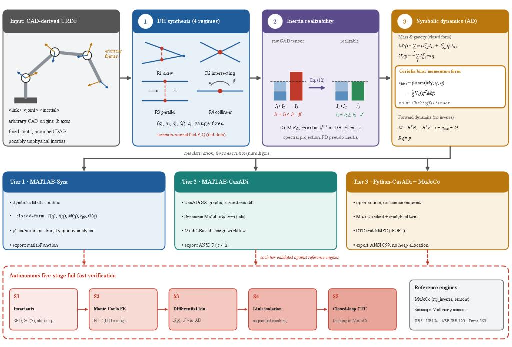
\includegraphics[width=\textwidth]{fig1_tri_paradigm_architecture.pdf}
	\caption{\textbf{Three-Tier System Architecture and Computational Pipeline.} Raw CAD-derived URDF descriptions (with arbitrary coordinate frames and unphysical CAD inertias) undergo: \textbf{(1) DH Synthesis across 4 Regimes:} resolving continuous gauge freedoms for skew (R1), intersecting (R2), parallel (R3), and collinear (R4) joint axes via common-normal feet $P, Q$ and automated axis-sign detection $s_i$; \textbf{(2) Inertia Realizability Projection:} spectral mapping of raw CAD inertia tensors onto the physically realizable set, enforcing the rigid-body triangle inequality ($I_1 + I_2 \ge I_3$) and positive-definite pseudo-inertias; \textbf{(3) Symbolic Dynamics via Algorithmic Differentiation:} closed-form mass metric $\bm{M}(\bm{q})$ and gravity $\bm{G}(\bm{q})$, generalized momentum directional derivative $\mathbf{c}_{\text{bias}}(\bm{q},\dot{\bm{q}}) = \operatorname{jtimes}(\bm{M}\dot{\bm{q}}, \bm{q}, \dot{\bm{q}}) - \frac{1}{2}\nabla_{\bm{q}}(\dot{\bm{q}}^T\bm{M}\dot{\bm{q}})$ eliminating $n^3$ Christoffel tensors, and Cholesky forward dynamics without explicit matrix inversion ($\bm{M} = \bm{R}^T\bm{R}$). The unified derivation branches into three complementary execution tiers: \textbf{Tier~1 (\texttt{MATLAB-Sym})} for glass-box algebraic inspectability and Lyapunov analysis; \textbf{Tier~2 (\texttt{MATLAB-CasADi})} for Simscape Multibody Model-Based Design; and \textbf{Tier~3 (\texttt{Python-MuJoCo})} for open-source nonlinear control (CTC and NMPC under IPOPT) with bare-metal ANSI C99 export. All tiers are validated against a \textbf{Five-Stage Verification Procedure} (S1: Physical invariants; S2: Monte Carlo forward kinematics; S3: Differential kinematics $\bm{J}, \dot{\bm{J}}$; S4: Sequential link inertia/gravity isolation; S5: Closed-loop CTC tracking in MuJoCo) cross-referenced against industrial platforms.}
	\label{fig:fig1_architecture}
\end{figure*}
	
	%==============================================================================
	\section{Analytical Framework for Kinematic and Dynamic Modeling of Serial Manipulators} \label{sec:methodology}
	%==============================================================================
	The objective of this section is to transform a raw robot description into a complete, executable dynamic model without requiring any manual derivation. The modeling procedure follows the natural sequence dictated by the underlying physics. A URDF file represents a robot as a tree of links and joints whose frame placements and axis orientations are selected primarily for CAD representation rather than analytical modeling. Therefore, the serial chain of actuated joints is first identified, and its geometry is expressed in the canonical DH convention. Particular attention is given to degenerate configurations, such as parallel or collinear joint axes, for which the convention is not unique. It is further demonstrated that the selected conventions in these cases do not affect the resulting kinematic description. Once the geometric structure has been established, the mass properties of each link are expressed in the corresponding frames and verified for physical consistency, since inertial parameters exported from CAD software are often inconsistent. The corrected inertial data are then combined with the kinematic description to construct the inertial and gravitational components of the equations of motion. Subsequently, the velocity-dependent Coriolis and centrifugal terms are derived from the time derivative of the generalized momentum through algorithmic differentiation. This approach remains mathematically equivalent to the classical formulation while avoiding its computationally expensive symbolic expansion. Finally, joint accelerations are obtained by factorizing the manipulator inertia matrix and solving the resulting system through triangular substitution rather than explicit matrix inversion. The resulting framework provides an efficient, numerically robust, and fully symbolic forward-dynamics model that is generated automatically from the URDF description.
	\subsection{Kinematic Chain Extraction and Denavit--Hartenberg Parameter Synthesis}
	\label{subsec:dh_synthesis}
	Transforming an arbitrary URDF into a valid analytical model begins with topological graph parsing and geometric axis alignment. Given an input URDF XML file, an entity-guarded parser constructs a directed acyclic graph $\mathcal{G} = (\mathcal{V}, \mathcal{E})$, where vertices $\mathcal{V} = \{L_0, \dots, L_M\}$ denote rigid links and directed edges $\mathcal{E} = \{J_1, \dots, J_M\}$ represent kinematic joints defined by parent-to-child homogeneous transformations $\bm{T}_{\text{joint},k}(\bm{t}_k, \bm{\varphi}_k) \in SE(3)$ and local actuation unit axes $\hat{\bm{u}}_k \in S^2$ \cite{ihab2026urdf2dt}.
	
	The structural base link $L_0$ is isolated via set difference between parent and child vertex sets. A breadth-first search traversing from $L_0$ extracts the ordered active serial chain $\mathcal{K} = \{(L_0, J_1, L_1), \dots, (L_{n-1}, J_n, L_n)\}$ containing $n$ actuated joints with joint type indicators $\sigma_i \in \{1\text{ (revolute)}, 0\text{ (prismatic)}\}$. Intermediate non-actuated connections ($\text{type} = \text{fixed}$) along the chain are topologically contracted: their relative homogeneous transformations and inertial tensors are folded into the nearest upstream active link via rigid-body parallel-axis transformations \cite{ihab2026urdf2dt}.
	
	At the home configuration ($\bm{q} = \bm{0}$), let $\bm{O}_{i-1}, \bm{O}_i \in \mathbb{R}^3$ denote the global origins of consecutive active joints $i-1$ and $i$, and let $\hat{\bm{z}}_{i-1}, \hat{\bm{z}}_i \in S^2$ denote their unit joint axes expressed in base coordinates $\{\mathcal{F}_0\}$. Defining the origin displacement $\Delta \bm{o}_i = \bm{O}_i - \bm{O}_{i-1}$, the cross-product magnitude $\delta_\times = \|\hat{\bm{z}}_{i-1} \times \hat{\bm{z}}_i\|_2$, and the normal separation distance yields the geometric classification metrics \cite{ihab2026urdf2dt}:
	\begin{equation}
		d_{\min} = \frac{|\Delta \bm{o}_i \cdot (\hat{\bm{z}}_{i-1} \times \hat{\bm{z}}_i)|}{\delta_\times} \quad (\delta_\times > \epsilon_\parallel), \qquad 
		d_\perp = \|\Delta \bm{o}_i - (\Delta \bm{o}_i \cdot \hat{\bm{z}}_{i-1})\hat{\bm{z}}_{i-1}\|_2 \quad (\delta_\times \le \epsilon_\parallel).
		\label{eq:dh_metrics}
	\end{equation}
	Using numerical thresholds $\epsilon_\parallel = 10^{-5}$ and $\epsilon_\cap = 10^{-6}$~m, each consecutive axis pair $(\hat{\bm{z}}_{i-1}, \hat{\bm{z}}_i)$ is classified into one of four canonical geometric regimes to compute the foot-points $\bm{P}_{i-1} \in \mathcal{L}_{i-1}(\bm{O}_{i-1}, \hat{\bm{z}}_{i-1})$ and $\bm{Q}_i \in \mathcal{L}_i(\bm{O}_i, \hat{\bm{z}}_i)$ defining the common normal line segment:
	\begin{enumerate}
		\item \textbf{Regime 1 (General Skew Axes, $\delta_\times > \epsilon_\parallel, \, d_{\min} > \epsilon_\cap$):} The spatial lines $\mathcal{L}_{i-1}(s) = \bm{O}_{i-1} + s\hat{\bm{z}}_{i-1}$ and $\mathcal{L}_i(t) = \bm{O}_i + t\hat{\bm{z}}_i$ admit a unique shortest perpendicular with no gauge freedom. Minimizing the squared Euclidean distance $\|\mathcal{L}_{i-1}(s) - \mathcal{L}_i(t)\|_2^2$ yields the unconstrained $2 \times 2$ linear system:
		\begin{equation}
			\begin{bmatrix} s^* \\ t^* \end{bmatrix} = \frac{1}{1 - (\hat{\bm{z}}_{i-1} \cdot \hat{\bm{z}}_i)^2} \begin{bmatrix} 1 & \hat{\bm{z}}_{i-1} \cdot \hat{\bm{z}}_i \\ \hat{\bm{z}}_{i-1} \cdot \hat{\bm{z}}_i & 1 \end{bmatrix} \begin{bmatrix} \Delta \bm{o}_i \cdot \hat{\bm{z}}_{i-1} \\ -\Delta \bm{o}_i \cdot \hat{\bm{z}}_i \end{bmatrix},
			\label{eq:pq_skew}
		\end{equation}
		providing the foot-points $\bm{P}_{i-1} = \bm{O}_{i-1} + s^*\hat{\bm{z}}_{i-1}$ and $\bm{Q}_i = \bm{O}_i + t^*\hat{\bm{z}}_i$, with normal axis $\hat{\bm{x}}_i = (\bm{Q}_i - \bm{P}_{i-1}) / \|\bm{Q}_i - \bm{P}_{i-1}\|_2$.
		
		\item \textbf{Regime 2 (Intersecting Axes, $\delta_\times > \epsilon_\parallel, \, d_{\min} \le \epsilon_\cap$):} The axes intersect at a single physical point $\bm{P}_{i-1} = \bm{Q}_i$ (enforcing link length $a_i = 0$) computed via Eq.~\eqref{eq:pq_skew}. The common normal direction is uniquely determined by $\hat{\bm{x}}_i = (\hat{\bm{z}}_{i-1} \times \hat{\bm{z}}_i) / \|\hat{\bm{z}}_{i-1} \times \hat{\bm{z}}_i\|_2$.
		
		\item \textbf{Regime 3 (Parallel Non-Collinear Axes, $\delta_\times \le \epsilon_\parallel, \, d_\perp > \epsilon_\cap$):} Because the axes are parallel, Eq.~\eqref{eq:pq_skew} becomes singular due to a continuous translational gauge freedom along $\hat{\bm{z}}_{i-1}$. The canonical solver resolves this ambiguity by anchoring $s^* = \lambda_i$ (defaulting to $\lambda_i = 0$, setting $\bm{P}_{i-1} = \bm{O}_{i-1}$), projecting orthogonally onto $\mathcal{L}_i$ via $t^* = (\bm{P}_{i-1} - \bm{O}_i) \cdot \hat{\bm{z}}_i$, setting $\bm{Q}_i = \bm{O}_i + t^*\hat{\bm{z}}_i$, and defining $\hat{\bm{x}}_i = (\bm{Q}_i - \bm{P}_{i-1}) / \|\bm{Q}_i - \bm{P}_{i-1}\|_2$.
		
		\item \textbf{Regime 4 (Collinear Axes, $\delta_\times \le \epsilon_\parallel, \, d_\perp \le \epsilon_\cap$):} The joint axes coincide ($a_i = 0, \, \alpha_i \in \{0, \pi\}$), admitting both translational gauge freedom $\lambda_i \in \mathbb{R}$ and rotational gauge freedom $\phi_i \in [-\pi, \pi)$ about $\hat{\bm{z}}_{i-1}$. The canonical solver sets $\bm{P}_{i-1} = \bm{Q}_i = \bm{O}_{i-1}$ and aligns the normal orientation with the preceding frame via $\hat{\bm{x}}_i = \operatorname{Rot}_z(\phi_i)\hat{\bm{x}}_{i-1}$ (with default canonical choice $\phi_i = 0$).
	\end{enumerate}
	
	From the synthesized orthonormal frames $\bm{R}_i^{\text{DH}} = [\hat{\bm{x}}_i, \, \hat{\bm{z}}_i \times \hat{\bm{x}}_i, \, \hat{\bm{z}}_i] \in SO(3)$ and origins $\bm{O}_i^{\text{DH}} = \bm{Q}_i$, the four classical DH parameters are extracted analytically:
	\begin{align}
		a_i &= (\bm{Q}_i - \bm{P}_{i-1}) \cdot \hat{\bm{x}}_i, & \alpha_i &= \operatorname{atan2}\!\left( (\hat{\bm{z}}_{i-1} \times \hat{\bm{z}}_i) \cdot \hat{\bm{x}}_i, \, \hat{\bm{z}}_{i-1} \cdot \hat{\bm{z}}_i \right), \label{eq:dh_a_alpha} \\
		d_i &= (\bm{P}_{i-1} - \bm{O}_{i-1}^{\text{DH}}) \cdot \hat{\bm{z}}_{i-1}, & \theta_i^{\text{off}} &= \operatorname{atan2}\!\left( (\hat{\bm{x}}_{i-1} \times \hat{\bm{x}}_i) \cdot \hat{\bm{z}}_{i-1}, \, \hat{\bm{x}}_{i-1} \cdot \hat{\bm{x}}_i \right). \label{eq:dh_d_theta}
	\end{align}
	These parameters yield the standard link transformation matrix $\bm{A}_i(q_i) = \operatorname{Rot}_z(\theta_i)\operatorname{Trans}_z(d_i)\operatorname{Trans}_x(a_i)\operatorname{Rot}_x(\alpha_i) \in SE(3)$:
	\begin{equation}
		\bm{A}_i(q_i) = \begin{bmatrix}
			\cos\theta_i & -\sin\theta_i\cos\alpha_i & \sin\theta_i\sin\alpha_i & a_i\cos\theta_i \\
			\sin\theta_i & \cos\theta_i\cos\alpha_i & -\cos\theta_i\sin\alpha_i & a_i\sin\theta_i \\
			0 & \sin\alpha_i & \cos\alpha_i & d_i \\
			0 & 0 & 0 & 1
		\end{bmatrix},
		\label{eq:dh_matrix}
	\end{equation}
	where $\theta_i = \theta_i^{\text{off}} + \sigma_i s_i q_i$ and $d_i = d_i^{\text{off}} + (1-\sigma_i) s_i q_i$. The scalar $s_i = \operatorname{sgn}(\operatorname{round}(\hat{\bm{u}}_i^{\text{urdf}} \cdot \hat{\bm{z}}_{i-1}^{\text{DH}})) \in \{-1, +1\}$ denotes the autonomously detected joint actuation parity factor.
	
	\begin{proposition}[Forward-Kinematic Gauge Invariance]
		\label{prop:gauge_invariance}
		Let $\bm{T}_0^n(\bm{q}) = \bm{A}_1(q_1)\cdots\bm{A}_n(q_n)\bm{T}_{\text{tool}}$ denote the global forward kinematics of a serial chain. If any intermediate frame $\mathcal{F}_i^{\text{DH}}$ ($1 \le i < n$) classified under Regime~3 or~4 undergoes an admissible gauge shift $\bm{T}_i' = \bm{T}_i \bm{\Delta}_i$, where $\bm{\Delta}_i = \operatorname{Trans}_z(\Delta d_i)\operatorname{Rot}_z(\Delta \theta_i)$ (with $\Delta \theta_i = 0$ in Regime~3), then updating the adjacent transformations via $\bm{A}_i'(q_i) = \bm{A}_i(q_i)\bm{\Delta}_i$ and $\bm{A}_{i+1}'(q_{i+1}) = \bm{\Delta}_i^{-1}\bm{A}_{i+1}(q_{i+1})$ preserves the standard DH geometric rules and leaves the end-effector pose $\bm{T}_0^n(\bm{q})$ invariant for all $\bm{q} \in \mathbb{R}^n$.
	\end{proposition}
	
	\begin{proof}
		Because joint $i+1$ acts strictly along $\hat{\bm{z}}_i$, the spatial perturbation matrix $\bm{\Delta}_i = \operatorname{Trans}_z(\Delta d_i)\operatorname{Rot}_z(\Delta \theta_i)$ belongs to the cylindrical subgroup $C(\hat{\bm{z}}_i) \subset SE(3)$. This subgroup commutes with the joint actuation operator $\bm{E}_{z}(q_{i+1}) \in \{\operatorname{Rot}_z(q_{i+1}), \operatorname{Trans}_z(q_{i+1})\}$, such that $\bm{\Delta}_i^{-1} \bm{E}_z(q_{i+1}) = \bm{E}_z(q_{i+1})\bm{\Delta}_i^{-1}$. Consequently, the product of adjacent transformations satisfies:
		\begin{equation}
			\bm{A}_i'(q_i)\bm{A}_{i+1}'(q_{i+1}) = \bm{A}_i(q_i)\bm{\Delta}_i \bm{\Delta}_i^{-1}\bm{A}_{i+1}(q_{i+1}) = \bm{A}_i(q_i)\bm{A}_{i+1}(q_{i+1})
		\end{equation}
		identically for all configuration states $(q_i, q_{i+1})$.
	\end{proof}
	
	\subsection{Inertial Parameters and Mass Matrix Assembly}
	\label{subsec:inertial_mapping}
	With the DH frames $\bm{T}_{0,\text{DH}}^i(\bm{0})$ synthesized, link inertial properties must be mapped from their local URDF definitions into the DH frame coordinates, validated for physical realizability, and then used to assemble the generalized mass matrix.
	
	\paragraph{Mapping into DH frames.}
	In the raw URDF, each link $i$ specifies a link mass $m_i$, local CoM position $\bm{c}_i^{\text{urdf}} \in \mathbb{R}^3$, inertial frame rotation $\bm{R}_{\text{ine},i} \in SO(3)$, and principal inertia tensor $\bm{I}_{\text{raw},i} \in \mathbb{R}^{3 \times 3}$. The raw inertia tensor is first rotated into the local URDF link frame via:
	\begin{equation}
		\bm{I}_i^{\text{urdf}} = \bm{R}_{\text{ine},i} \, \bm{I}_{\text{raw},i} \, \bm{R}_{\text{ine},i}^T.
	\end{equation}
	
	Let $\bm{T}_{0,\text{urdf}}^i(\bm{0}) = \begin{bmatrix} \bm{R}_{u,i} & \bm{p}_{u,i} \\ \bm{0} & 1 \end{bmatrix}$ and $\bm{T}_{0,\text{DH}}^i(\bm{0}) = \begin{bmatrix} \bm{R}_{d,i} & \bm{p}_{d,i} \\ \bm{0} & 1 \end{bmatrix}$ denote the zero-configuration base poses of URDF link $i$ and synthesized DH frame $i$, respectively. The link CoM position in base coordinates is $\bm{p}_{C_i}^0(\bm{0}) = \bm{p}_{u,i} + \bm{R}_{u,i}\bm{c}_i^{\text{urdf}}$. 
	
	Following our unified DH convention \cite{ihab2026urdf2dt, asr2026calibration}, we define $\bm{P}_{C_i} \in \mathbb{R}^3$ as the CoM position vector of link $i$ relative to the preceding DH origin $\bm{p}_{d,i-1}$, expressed in the orientation of DH frame $i$. The rotational inertia tensor aligned with DH frame $i$ is then computed as:
	\begin{align}
		\bm{P}_{C_i} &= \bm{R}_{d,i}^T \left( \bm{p}_{C_i}^0(\bm{0}) - \bm{p}_{d,i-1} \right), \label{eq:com_dh_map} \\
		\bm{I}_i^{\text{DH}} &= \bm{R}_{\text{rel},i} \, \bm{I}_i^{\text{urdf}} \, \bm{R}_{\text{rel},i}^T, \quad \text{where } \bm{R}_{\text{rel},i} = \bm{R}_{d,i}^T \bm{R}_{u,i} \in SO(3). \label{eq:inertia_dh_map}
	\end{align}
	
	\paragraph{Physical consistency of inertia tensors.}
	To ensure physical consistency across models obtained from diverse CAD sources, the mapped inertia tensors are validated against rigid-body realizability conditions. A symmetric matrix $\bm{I}_i^{\text{DH}} \in \mathbb{S}^3$ represents a physically realizable rigid body of non-negative mass density $\rho(\bm{r}) \ge 0$ if and only if its principal eigenvalues $0 < I_1 \le I_2 \le I_3$, obtained from the spectral decomposition $\bm{I}_i^{\text{DH}} = \bm{V}\operatorname{diag}(I_1, I_2, I_3)\bm{V}^T$ with $\bm{V} \in SO(3)$, satisfy strict positivity and the triangle inequality $I_1 + I_2 \ge I_3$ \cite{sousa2019physical}. This is equivalent to requiring that the pseudo-inertia matrix $\bm{\mathcal{J}}_i = \frac{1}{2}\operatorname{tr}(\bm{I}_i^{\text{DH}})\bm{I}_3 - \bm{I}_i^{\text{DH}}$ be strictly positive-definite ($\bm{\mathcal{J}}_i \succ \bm{0}$).
	
	When a URDF link tensor violates these conditions, our framework projects its eigenvalues onto the realizable cone:
	\begin{equation}
		\tilde{I}_k = \max(I_k, \, \epsilon_{\text{eig}}) \quad (k=1,2,3), \qquad 
		\hat{I}_3 = \min\!\left(\tilde{I}_3, \, \tilde{I}_1 + \tilde{I}_2 - \epsilon_{\text{tri}}\right), \qquad 
		\hat{\bm{I}}_i^{\text{DH}} = \bm{V}\operatorname{diag}(\tilde{I}_1, \tilde{I}_2, \hat{I}_3)\bm{V}^T,
		\label{eq:spectral_sanitization}
	\end{equation}
	where $\epsilon_{\text{eig}} = 10^{-7}$~kg$\cdot$m$^2$ and $\epsilon_{\text{tri}} = 10^{-9}$~kg$\cdot$m$^2$ provide numerical feasibility margins. For tensors that already satisfy the conditions, $\hat{\bm{I}}_i^{\text{DH}} = \bm{I}_i^{\text{DH}}$, and the sanitized tensors $\hat{\bm{I}}_i^{\text{DH}}$ are used in all subsequent dynamic computations.
	
	\paragraph{Spatial Jacobians and mass matrix assembly.}
	At an arbitrary configuration $\bm{q} \in \mathbb{R}^n$, forward kinematic evaluation $\bm{T}_0^i(\bm{q}) = \bm{T}_0^{i-1}(\bm{q})\bm{A}_i(q_i)$ yields the link orientation $\bm{R}_0^i(\bm{q}) = [\bm{T}_0^i]_{1:3,1:3}$, joint rotation axis $\bm{z}_{j-1}(\bm{q}) = [\bm{T}_0^{j-1}]_{1:3,3}$, origin location $\bm{p}_{j-1}(\bm{q}) = [\bm{T}_0^{j-1}]_{1:3,4}$, and link CoM position in the base frame:
	\begin{equation}
		\bm{p}_{C_i}^0(\bm{q}) = \bm{p}_{i-1}(\bm{q}) + \bm{R}_0^i(\bm{q})\bm{P}_{C_i}, \qquad \bm{r}_{j,C_i}(\bm{q}) = \bm{p}_{C_i}^0(\bm{q}) - \bm{p}_{j-1}(\bm{q}) \quad (j \le i).
		\label{eq:com_forward}
	\end{equation}
	
	The translational Jacobian $\bm{J}_{v,i}(\bm{q}) \in \mathbb{R}^{3 \times n}$ and rotational Jacobian $\bm{J}_{\omega,i}(\bm{q}) \in \mathbb{R}^{3 \times n}$ for link $i$ are constructed column-wise for $j \in \{1, \dots, n\}$ using joint type indicators $\sigma_j \in \{0, 1\}$:
	\begin{equation}
		\bm{J}_{v,i}(:,j) = \begin{cases}
			\sigma_j \left(\bm{z}_{j-1} \times \bm{r}_{j,C_i}\right) + (1 - \sigma_j)\bm{z}_{j-1}, & j \le i, \\
			\bm{0}_{3 \times 1}, & j > i,
		\end{cases} \qquad
		\bm{J}_{\omega,i}(:,j) = \begin{cases}
			\sigma_j \bm{z}_{j-1}, & j \le i, \\
			\bm{0}_{3 \times 1}, & j > i.
		\end{cases}
		\label{eq:link_jacobians}
	\end{equation}
	Rotating each sanitized link inertia tensor into the base frame via $\bm{I}_i^0(\bm{q}) = \bm{R}_0^i(\bm{q}) \hat{\bm{I}}_i^{\text{DH}} \bm{R}_0^i(\bm{q})^T$ yields the closed-form generalized mass matrix $\bm{M}(\bm{q})$ and gravitational torque vector $\bm{G}(\bm{q})$:
	\begin{equation}
		\bm{M}(\bm{q}) = \sum_{i=1}^n \left( m_i \bm{J}_{v,i}^T \bm{J}_{v,i} + \bm{J}_{\omega,i}^T \bm{I}_i^0 \bm{J}_{\omega,i} \right), \qquad 
		\bm{G}(\bm{q}) = -\sum_{i=1}^n \bm{J}_{v,i}^T m_i \bm{g}.
		\label{eq:M_and_G}
	\end{equation}
	
	\subsection{Coriolis and Centrifugal Terms via Momentum Derivatives}
	\label{subsec:momentum_derivative}
	For an $n$-DOF serial manipulator with kinetic energy $T(\bm{q}, \dot{\bm{q}}) = \frac{1}{2}\dot{\bm{q}}^T\bm{M}(\bm{q})\dot{\bm{q}}$ and potential energy $V(\bm{q}) = -\sum_{i=1}^n m_i \bm{g}^T \bm{p}_{C_i}^0(\bm{q})$, the Euler--Lagrange equations of motion are expressed as:
	\begin{equation}
		\frac{d}{dt}\left(\frac{\partial T}{\partial \dot{\bm{q}}}\right) - \nabla_{\bm{q}} T(\bm{q}, \dot{\bm{q}}) + \nabla_{\bm{q}} V(\bm{q}) = \bm{\tau}.
		\label{eq:el_vector}
	\end{equation}
	
	Defining the generalized momentum $\bm{p} \equiv \nabla_{\dot{\bm{q}}} T = \bm{M}(\bm{q})\dot{\bm{q}}$, its time derivative along state trajectories is given by:
	\begin{equation}
		\frac{d}{dt}\bm{p}(\bm{q}, \dot{\bm{q}}) = \bm{M}(\bm{q})\ddot{\bm{q}} + \left(\frac{\partial (\bm{M}(\bm{q})\dot{\bm{q}})}{\partial \bm{q}}\right)\dot{\bm{q}}.
		\label{eq:momentum_time_deriv}
	\end{equation}
	Substituting Eq.~\eqref{eq:momentum_time_deriv} into Eq.~\eqref{eq:el_vector} isolates the Coriolis and centrifugal bias vector $\mathbf{c}_{\text{bias}}(\bm{q}, \dot{\bm{q}})$:
	\begin{equation}
		\mathbf{c}_{\text{bias}}(\bm{q}, \dot{\bm{q}}) \equiv \left(\frac{\partial (\bm{M}(\bm{q})\dot{\bm{q}})}{\partial \bm{q}}\right)\dot{\bm{q}} - \frac{1}{2}\nabla_{\bm{q}}\!\left(\dot{\bm{q}}^T \bm{M}(\bm{q})\dot{\bm{q}}\right).
		\label{eq:cbias_exact}
	\end{equation}
	
	The first term in Eq.~\eqref{eq:cbias_exact} is evaluated as a directional derivative (Jacobian-vector product, JVP) via forward-mode algorithmic differentiation, while the second term is computed as the gradient of scalar kinetic energy via reverse-mode algorithmic differentiation.
	
	\begin{proposition}[Algebraic Equivalence to Classical Christoffel Form]
		\label{prop:christoffel_equiv}
		Let $\bm{C}(\bm{q}, \dot{\bm{q}}) \in \mathbb{R}^{n \times n}$ denote the classical Coriolis matrix with entries defined via Christoffel symbols of the first kind:
		\begin{equation}
			\left[\bm{C}(\bm{q},\dot{\bm{q}})\right]_{ij} = \sum_{k=1}^n \frac{1}{2}\left( \frac{\partial M_{ij}}{\partial q_k} + \frac{\partial M_{ik}}{\partial q_j} - \frac{\partial M_{kj}}{\partial q_i} \right) \dot{q}_k.
			\label{eq:christoffel_classical}
		\end{equation}
		Then, for all $(\bm{q}, \dot{\bm{q}}) \in \mathbb{R}^n \times \mathbb{R}^n$, the identity $\bm{C}(\bm{q}, \dot{\bm{q}})\dot{\bm{q}} \equiv \mathbf{c}_{\text{bias}}(\bm{q}, \dot{\bm{q}})$ holds, and the system satisfies the energy conservation condition $\dot{\bm{q}}^T(\dot{\bm{M}} - 2\bm{C})\dot{\bm{q}} = 0$.
	\end{proposition}
	
	\begin{proof}
		Expanding the $i$-th component of the classical vector product $\bm{C}(\bm{q}, \dot{\bm{q}})\dot{\bm{q}}$ yields:
		\begin{equation}
			\left[\bm{C}(\bm{q}, \dot{\bm{q}})\dot{\bm{q}}\right]_i = \frac{1}{2}\sum_{j=1}^n \sum_{k=1}^n \frac{\partial M_{ij}}{\partial q_k}\dot{q}_j\dot{q}_k + \frac{1}{2}\sum_{j=1}^n \sum_{k=1}^n \frac{\partial M_{ik}}{\partial q_j}\dot{q}_j\dot{q}_k - \frac{1}{2}\sum_{j=1}^n \sum_{k=1}^n \frac{\partial M_{kj}}{\partial q_i}\dot{q}_j\dot{q}_k.
		\end{equation}
		Exchanging summation indices $j \leftrightarrow k$ in the second term demonstrates equivalence with the first summation. Combining these terms yields:
		\begin{equation}
			\sum_{j=1}^n \sum_{k=1}^n \frac{\partial M_{ij}}{\partial q_k}\dot{q}_k\dot{q}_j = \left[\left(\frac{\partial (\bm{M}(\bm{q})\dot{\bm{q}})}{\partial \bm{q}}\right)\dot{\bm{q}}\right]_i.
		\end{equation}
		The remaining summation corresponds to the scalar kinetic energy gradient $-\frac{1}{2}\frac{\partial}{\partial q_i}(\dot{\bm{q}}^T\bm{M}(\bm{q})\dot{\bm{q}})$, confirming that $\bm{C}(\bm{q},\dot{\bm{q}})\dot{\bm{q}} \equiv \mathbf{c}_{\text{bias}}(\bm{q},\dot{\bm{q}})$. Taking the inner product with $\dot{\bm{q}}$ yields $\dot{\bm{q}}^T \mathbf{c}_{\text{bias}} = \frac{1}{2}\dot{\bm{q}}^T \dot{\bm{M}}\dot{\bm{q}}$, verifying trajectory-level energy conservation $\frac{d}{dt}T = \dot{\bm{q}}^T(\bm{\tau} - \bm{G})$.
	\end{proof}
	
	\begin{theorem}[Computational Complexity of Algorithmic Momentum Derivatives]
		\label{thm:complexity}
		Let $\operatorname{cost}(\bm{M}(\bm{q}))$ denote the computational complexity of evaluating the generalized mass matrix graph. While evaluating $\mathbf{c}_{\text{Christoffel}}$ via uncompressed Christoffel tensors scales as $\mathcal{O}(n^4)$ ($\mathcal{O}(n^{3.24})$ under compiler common subexpression elimination), evaluating the direct momentum formulation satisfies:
		\begin{equation}
			\operatorname{cost}(\mathbf{c}_{\text{bias}}(\bm{q},\dot{\bm{q}})) \le (c_f + c_r) \cdot \operatorname{cost}(\bm{M}(\bm{q})) + \mathcal{O}(n^2),
			\label{eq:ad_cost_bound}
		\end{equation}
		where $c_f \le 3$ is the forward-mode directional derivative constant and $c_r \le 4$ is the reverse-mode gradient constant. Thus, the evaluation cost of the Coriolis bias vector is asymptotically bounded by a constant factor of the mass matrix cost.
	\end{theorem}
	
	\begin{proof}
		Evaluating the generalized momentum $\bm{p} = \bm{M}(\bm{q})\dot{\bm{q}}$ requires one matrix-vector product with complexity $\operatorname{cost}(\bm{M}) + \mathcal{O}(n^2)$. By forward-mode algorithmic differentiation, the Jacobian-vector product $\left(\frac{\partial \bm{p}}{\partial \bm{q}}\right)\dot{\bm{q}}$ along the constant seed vector $\dot{\bm{q}}$ costs at most $c_f \cdot \operatorname{cost}(\bm{p})$ operations, where $c_f \le 3$. By the Baur--Strassen theorem, evaluating the kinetic energy gradient $\nabla_{\bm{q}} T$ via reverse-mode AD requires at most $c_r \cdot \operatorname{cost}(T)$ operations, where $c_r \le 4$. Summing these operational bounds yields Eq.~\eqref{eq:ad_cost_bound}.
	\end{proof}
	
	\begin{remark}[Mass Matrix Scaling and Empirical Complexity Bounds]
		Analytically, constructing $\bm{M}(\bm{q}) = \sum_{i=1}^n (m_i \bm{J}_{v,i}^T\bm{J}_{v,i} + \bm{J}_{\omega,i}^T \bm{I}_i^0 \bm{J}_{\omega,i})$ naively requires $\sum_{i=1}^n i^2 = \frac{n(n+1)(2n+1)}{6} = \mathcal{O}(n^3)$ operations. Under computer-algebra and algorithmic differentiation systems, compiler common subexpression elimination (CSE) automatically merges redundant trigonometric sub-trees across kinematic frames. Across our systematic scalability benchmark ($n \in [3, 14]$, Table~\ref{tab:table5_scalability}), power-law log-log regressions yield an empirical scaling exponent of $\alpha = 2.27 \pm 0.10$ ($R^2 = 0.9985$) for $\bm{M}(\bm{q})$ and $\alpha = 2.28 \pm 0.09$ ($R^2 = 0.9989$) for the proposed momentum bias vector $\mathbf{c}_{\text{bias}}$. This empirically confirms that $\operatorname{cost}(\mathbf{c}_{\text{bias}})$ scales as a constant multiple ($3.98 \pm 0.04\times$) of $\operatorname{cost}(\bm{M})$, in contrast to classical Christoffel evaluation which scales at $\alpha = 3.24 \pm 0.14$ ($R^2 = 0.9985$).
	\end{remark}
	
	\subsection{Forward Dynamics via Symbolic Cholesky Factorization}
	\label{subsec:cholesky_dynamics}
	\begin{proposition}[Guaranteed Positive-Definiteness and Cholesky Dynamics]
		\label{prop:cholesky}
		For any serial kinematic chain with positive link masses $m_i > 0$ and realizable inertia tensors $\bm{I}_i^{\text{DH}} \succ \bm{0}$, if each joint axis $\bm{z}_{i-1}$ acts non-trivially on link $i$, then $\bm{M}(\bm{q}) \succ \bm{0}$ is strictly symmetric positive-definite for all $\bm{q} \in \mathbb{R}^n$. Consequently, $\bm{M}(\bm{q})$ admits a unique, pivot-free symbolic Cholesky decomposition $\bm{M}(\bm{q}) = \bm{R}(\bm{q})^T\bm{R}(\bm{q})$, where $\bm{R}(\bm{q})$ is an upper-triangular matrix with positive diagonal entries:
		\begin{equation}
			R_{ii}(\bm{q}) = \sqrt{M_{ii}(\bm{q}) - \sum_{k=1}^{i-1} R_{ki}(\bm{q})^2} > 0.
		\end{equation}
		Forward dynamics $\ddot{\bm{q}} = \bm{M}(\bm{q})^{-1}(\bm{\tau} - \mathbf{c}_{\text{bias}} - \bm{G})$ can therefore be resolved in $\frac{1}{3}n^3 + 2n^2$ operations via two successive triangular substitution passes:
		\begin{equation}
			\bm{R}(\bm{q})^T \bm{y} = \bm{\tau} - \mathbf{c}_{\text{bias}}(\bm{q},\dot{\bm{q}}) - \bm{G}(\bm{q}), \qquad \bm{R}(\bm{q})\ddot{\bm{q}} = \bm{y}.
			\label{eq:cholesky_solve}
		\end{equation}
	\end{proposition}

%==============================================================================
\section{Model Predictive Control and Software Implementation}
\label{sec:control_arch}
%==============================================================================

Having established the dynamic model, we assess its usefulness in a demanding real-time setting. The model is embedded in a predictive controller that repeatedly solves a constrained trajectory optimization problem over a short future horizon, applies only the first control action, and solves again from the newly measured state. Because the optimization solver must differentiate the dynamics many times per iteration, the cost of evaluating the model and its derivatives directly determines the achievable control rate, which is why the efficiency of the model derived above matters in this application. This section also describes how the same model is exported to several software environments, ranging from human-readable expressions for theoretical analysis, through compiled code for digital-twin simulation, to high-speed runtimes for real-time control, so that a single description serves analysis, simulation, and deployment.

\subsection{Receding-Horizon Nonlinear Model Predictive Control}
\label{subsec:nmpc}
To assess real-time utility, the derived dynamics model is integrated into a continuous-time constrained Optimal Control Problem (OCP) across a prediction horizon $T_h$:
\begin{align}
	\min_{\bm{x}(\cdot), \bm{u}(\cdot)} & \int_0^{T_h} \left( \|\bm{x}(t) - \bm{x}_{\text{ref}}(t)\|_{\bm{W}_x}^2 + \|\bm{u}(t)\|_{\bm{W}_u}^2 \right) dt + \|\bm{x}(T_h) - \bm{x}_{\text{ref}}(T_h)\|_{\bm{W}_T}^2 \label{eq:nmpc_ocp} \\
	\text{subject to } & \dot{\bm{x}}(t) = \begin{bmatrix} \dot{\bm{q}}(t) \\ \bm{R}(\bm{q})^{-1}\bm{R}(\bm{q})^{-T}\left(\bm{u}(t) - \mathbf{c}_{\text{bias}}(\bm{q},\dot{\bm{q}}) - \bm{G}(\bm{q})\right) \end{bmatrix}, \quad \bm{x}(0) = \bm{x}_{\text{meas}}, \label{eq:nmpc_dyn} \\
	& \bm{u}_{\min} \le \bm{u}(t) \le \bm{u}_{\max}, \quad \bm{x}_{\min} \le \bm{x}(t) \le \bm{x}_{\max}, \label{eq:nmpc_bounds} \\
	& \|\bm{p}_{\text{ee}}(\bm{q}(t)) - \bm{p}_{\text{obs}}\|_2 \ge r_{\text{obs}} + d_{\text{safe}}, \label{eq:nmpc_obs}
\end{align}
where $\bm{x} = [\bm{q}^T, \dot{\bm{q}}^T]^T \in \mathbb{R}^{2n}$, $\bm{u} = \bm{\tau} \in \mathbb{R}^n$, and $\bm{W}_x$, $\bm{W}_u$, $\bm{W}_T$ are the state, input, and terminal weighting matrices. In Eq.~\eqref{eq:nmpc_dyn}, the products with $\bm{R}(\bm{q})^{-1}$ and $\bm{R}(\bm{q})^{-T}$ are realized by the two triangular substitution passes of Eq.~\eqref{eq:cholesky_solve} and never as explicit matrix inverses.

The continuous problem is transcribed using direct multiple shooting over $N$ intervals, enforcing continuity via fourth-order Runge--Kutta (RK4) integration constraints $\bm{g}_k(\bm{x}_k, \bm{u}_k, \bm{x}_{k+1}) = \bm{x}_{k+1} - \bm{\phi}_{\text{RK4}}(\bm{x}_k, \bm{u}_k, \Delta t) = \bm{0}$. The resulting nonlinear program is resolved through primal-dual interior-point iterations on the Karush--Kuhn--Tucker (KKT) system:
\begin{equation}
	\begin{bmatrix} \nabla_{\bm{w}\bm{w}}^2 \mathcal{L} + \bm{\Sigma} & \nabla_{\bm{w}} \bm{g}^T \\ \nabla_{\bm{w}} \bm{g} & \bm{0} \end{bmatrix} \begin{bmatrix} \Delta \bm{w} \\ \Delta \bm{\lambda} \end{bmatrix} = - \begin{bmatrix} \nabla_{\bm{w}} \mathcal{L} \\ \bm{g}(\bm{w}) \end{bmatrix}.
	\label{eq:kkt_system}
\end{equation}
Because evaluating the stage sensitivities $\partial \bm{\phi}_{\text{RK4}}/\partial \bm{x}_k$ and $\partial \bm{\phi}_{\text{RK4}}/\partial \bm{u}_k$ requires differentiating the underlying forward dynamics graph, replacing explicit matrix inversion with triangular substitution and compacting the symbolic dynamics graph from 15,814 to 7,041 instructions (a $55.4\%$ reduction) directly cuts algorithmic differentiation time across the KKT matrix.

\subsection{Code Generation and Multi-Platform Deployment}
\label{subsec:codegen_tiers}
To accommodate diverse robotics applications, the pipeline compiles the symbolic model for three target tiers:
\begin{itemize}
	\item \textbf{Tier 1 (\texttt{MATLAB-Sym}):} Human-interpretable symbolic expressions generated via the MATLAB Symbolic Math Toolbox, retaining full skew-symmetric matrix representations for Lyapunov stability analysis and theoretical synthesis.
	\item \textbf{Tier 2 (\texttt{MATLAB-CasADi}):} Compressed directed acyclic graphs (DAGs) compiled to ANSI C code, combined with automated scripts (\texttt{dt\_build.m}) that programmatically assemble a 1:1 physical digital twin in Simscape Multibody.
	\item \textbf{Tier 3 (\texttt{Python-MuJoCo}):} High-performance compiled C runtimes interfaced with Python and headless MuJoCo physics engines, supporting dual-twin co-simulation and real-time NMPC updates at frequencies exceeding $1$~kHz.
\end{itemize}

%==============================================================================
\section{Validation Protocol and Benchmark Platforms}
\label{sec:validation}
%==============================================================================

To establish that automatically generated models are correct, physically consistent, and usable for control, the pipeline is applied to four industrial manipulators chosen to span different geometries, wrist designs, and payload classes. Each synthesized model is then subjected to a graded sequence of automated checks. The sequence begins with basic physical and algebraic properties of the model, continues with kinematics and their derivatives, compares the dynamic terms link by link against independent physics simulators, and ends with closed-loop trajectory tracking. Ordering the checks from the most elementary to the most integrated allows any failure to be traced to the stage where it first appears, while a model that passes every stage is consistent both with the underlying physics and with the reference simulators.

\subsection{Benchmark Manipulators}
\label{subsec:benchmark_platforms}
The proposed pipeline was evaluated across four industrial manipulators covering various kinematic configurations, spherical and non-spherical wrists, and payload classes:
\begin{enumerate}
	\item \textbf{Universal Robots UR5 (Medium-Reach Cobot):} 6-DOF architecture ($18.40$~kg mass, $0.850$~m reach) featuring parallel shoulder and elbow axes with an orthogonal, non-spherical wrist ($d_4 = 0.1091$~m, $d_5 = 0.0946$~m, $a_6 = 0.0823$~m).
	\item \textbf{Universal Robots UR16e (Heavy-Payload Cobot):} 6-DOF architecture ($33.10$~kg mass, $0.900$~m reach, $16.0$~kg payload) characterized by massive proximal links ($m_2 = 10.45$~kg, $m_3 = 4.32$~kg) inducing pronounced nonlinear inertial cross-coupling.
	\item \textbf{ABB IRB 120 (Spherical-Wrist Arm):} 6-DOF compact manipulator ($25.00$~kg mass, $0.580$~m reach) exhibiting a spatial shoulder offset ($a_3 = 0.070$~m) and a canonical three-axis intersecting spherical wrist ($a_4 = a_5 = a_6 = 0$).
	\item \textbf{Unimation Puma 560 (Classical Benchmark):} 6-DOF spatial manipulator ($54.20$~kg mass, $0.864$~m reach) possessing kinematic shoulder offsets ($d_3 = 0.1501$~m, $a_3 = -0.0203$~m) and historical CAD inertial parameters requiring spectral sanitization.
\end{enumerate}

\subsection{Multi-Stage Verification Procedure}
\label{subsec:verification_suite}
To guarantee mathematical correctness and physical consistency, every synthesized model must pass five automated verification stages:

\begin{enumerate}
	\item \textbf{Stage 1: Physical and Algebraic Invariants.} Asserts strictly positive link masses ($m_i > 0$), verifies the spectral triangle inequality on the sanitized inertia tensors $\hat{\bm{I}}_i^{\text{DH}}$, checks rotation matrix orthogonality ($\|\bm{R}^T\bm{R} - \bm{I}\|_F < 10^{-10}$), guarantees mass matrix positive-definiteness ($\bm{M}(\bm{q}) \succ \bm{0}$), and validates static gravity equilibrium:
	\begin{equation}
		\|\bm{\tau}(\bm{q},\bm{0},\bm{0}) - \bm{G}(\bm{q})\|_\infty < 10^{-12}~\text{N}\cdot\text{m}.
	\end{equation}
	
	\item \textbf{Stage 2: Forward Kinematics Certification.} Compares end-effector position $\bm{p}_{\text{ee}}(\bm{q})$ and orientation quaternion $\bm{\xi}_{\text{ee}}(\bm{q})$ against MuJoCo and Simscape across 1,000 randomized configurations under reach-scaled tolerances:
	\begin{equation}
		\text{tol}_{\text{pos}} = \max\!\left(10^{-4}~\text{m}, \; 5 \times 10^{-4} \sum_{i=1}^n (|a_i| + |d_i|)\right).
	\end{equation}
	
	\item \textbf{Stage 3: Differential Kinematics and Derivatives.} Validates the spatial manipulator Jacobian $\bm{J}(\bm{q})$ and its exact AD time-derivative $\dot{\bm{J}}(\bm{q},\dot{\bm{q}})$ against central finite differences across velocity boundaries.
	
	\item \textbf{Stage 4: Sequential Inertia and Gravity Isolation.} Validates dynamic terms by sequentially isolating individual links. For each link stage $i \in \{1, \dots, n\}$, downstream inertial parameters are zeroed ($m_k = 0, \bm{I}_k = \bm{0}$ for $k > i$), and non-active joints are held stationary ($\dot{q}_j = \ddot{q}_j = 0$ for $j \neq i$):
	\begin{equation}
		\tau_i^{(i)}(t) = M_{ii}^{(i)}(\bm{q})\ddot{q}_i(t) + G_i^{(i)}(\bm{q}).
		\label{eq:isolated_link_torque}
	\end{equation}
	Because the scalar inertia $M_{ii}^{(i)}$ of an isolated link rotating about its own joint axis is invariant to $q_i$ ($\partial M_{ii}^{(i)}/\partial q_i \equiv 0$), inertial and gravitational torques are decoupled and validated directly against simulator readings.
	
	\item \textbf{Stage 5: Closed-Loop Computed Torque Trajectory Tracking.} Implements a feedback-linearizing controller with automated joint sign parity correction $\bm{S} = \operatorname{diag}(s_1, \dots, s_n) \in \{-1, +1\}^{n \times n}$:
	\begin{equation}
		\bm{\tau}(t) = \bm{S} \, \bm{\tau}_{\text{ana}}\!\left( \bm{S}\bm{q}(t), \, \bm{S}\dot{\bm{q}}(t), \, \bm{S}\left[\ddot{\bm{q}}_d(t) + \bm{K}_d(\dot{\bm{q}}_d - \dot{\bm{q}}) + \bm{K}_p(\bm{q}_d - \bm{q})\right] \right),
		\label{eq:ctc_law}
	\end{equation}
	ensuring global asymptotic tracking error convergence via the linear error system $\ddot{\bm{e}}(t) + \bm{K}_d\dot{\bm{e}}(t) + \bm{K}_p\bm{e}(t) = \bm{0}$.
\end{enumerate}
	
%==============================================================================
\section*{Results}
%==============================================================================

The results are organized around five testable hypotheses, each addressing a distinct claim about the proposed modeling pipeline. We first examine the computational cost of the generated dynamics model, measuring how much the reformulation of the velocity-dependent terms and the factorization-based forward dynamics shrink the symbolic computation graph and its execution time. We then verify that the geometric synthesis and the inertial correction handle manipulators of different architectures and manufacturers without manual tuning, and that the resulting models agree with independent physics simulators. Next, we study how the cost grows with the number of joints, to determine whether the observed savings persist in larger systems. The final two experiments test the model in closed loop: first in trajectory tracking with a model-based controller, and then within a predictive controller that must respect actuator limits and avoid an obstacle in the workspace. Each experiment begins with the hypothesis under test, describes the setup, and ends with the quantitative findings that support or refute it.

\subsection*{Computational Cost Reduction of the Dynamics Model}

\noindent\textbf{Hypothesis Tested:} \textit{Reformulating Coriolis and centrifugal effects via generalized momentum directional derivatives eliminates the combinatorial explosion of rank-3 Christoffel tensors, reducing symbolic instruction counts by over $50\%$ on 6-DOF industrial manipulators without numerical loss.}

To test this hypothesis, we profiled the complete symbolic Directed Acyclic Graph (DAG) for the heavy-payload Universal Robots UR16e ($n=6$) in CasADi. Table~\ref{tab:table3_opcodes} details the operation counts across individual dynamic components comparing the classical Christoffel baseline against our proposed momentum formulation.

\begin{table*}[!t]
	\caption{\textbf{Symbolic Graph Profiling and Instruction Breakdown on the UR16e 6-DOF Manipulator.}}
	\label{tab:table3_opcodes}
	\centering
	\small
	\begin{tabularx}{\textwidth}{p{2.3cm}p{4.1cm}ccc>{\raggedright\arraybackslash}X}
		\toprule
		\textbf{Dynamic Term} & \textbf{Mathematical Formulation} & \textbf{Complexity} & \textbf{Baseline Op.} & \textbf{Proposed Op.} & \textbf{Symbolic Graph Impact} \\
		\midrule
		Mass Matrix $\bm{M}(\bm{q})$ & $\sum_{i=1}^n (m_i \bm{J}_{v,i}^T \bm{J}_{v,i} + \bm{J}_{\omega,i}^T \bm{I}_i^0 \bm{J}_{\omega,i})$ & $O(n^2)$ & 2,190 & 2,190 & Kinetic metric tensor ($6 \times 6$ strictly SPD). \\
		Gravity Vector $\bm{G}(\bm{q})$ & $-\sum_{i=1}^n \bm{J}_{v,i}^T m_i \bm{g}$ & $O(n)$ & 334 & 334 & Closed-form gravitational torque vector in 3D. \\
		Coriolis Bias $\mathbf{c}_{\text{bias}}(\bm{q},\dot{\bm{q}})$ & $\left(\frac{\partial (\bm{M}\dot{\bm{q}})}{\partial \bm{q}}\right)\dot{\bm{q}} - \frac{1}{2}\nabla_{\bm{q}}(\dot{\bm{q}}^T\bm{M}\dot{\bm{q}})$ & $O(n^2)$ vs.\ $O(n^4)$ & 14,936 & 5,495 & \textbf{-63.2\% opcodes} (Forward JVP and reverse gradient replace 216 Christoffel derivatives). \\
		Inverse Dynamics $\bm{\tau}$ & $\bm{M}(\bm{q})\ddot{\bm{q}} + \mathbf{c}_{\text{bias}}(\bm{q},\dot{\bm{q}}) + \bm{G}(\bm{q})$ & $O(n^2)$ & 17,460 & 8,019 & \textbf{-54.1\% opcodes} ($108.8~\mu$s in Python, $9.19$~kHz throughput). \\
		Forward Dynamics $\ddot{\bm{q}}$ & $\bm{R}^T \bm{y} = \bm{\tau} - \mathbf{c}_{\text{bias}} - \bm{G}, \; \bm{R}\ddot{\bm{q}} = \bm{y}$ & $O(n^3)$ Cholesky & 15,814 & 7,041 & \textbf{-55.4\% opcodes} ($1.92\times$ speedup: $78.7~\mu$s bare-metal ANSI C / $99.2~\mu$s Python vs.\ $151.5~\mu$s; no explicit inversion). \\
		\bottomrule
	\end{tabularx}
\end{table*}

The empirical instruction audit confirms the hypothesis:
\begin{enumerate}
	\item \textbf{Coriolis Graph Compression:} Bypassing the $n^3 = 216$ Christoffel partial derivatives slashes Coriolis evaluation from $14,936$ to $5,495$ scalar instructions---\textbf{a $63.2\%$ reduction in opcodes}.
	\item \textbf{Forward Dynamics Compression:} Coupling the momentum Coriolis derivative with symbolic Cholesky factorization reduces total forward dynamics opcodes from $15,814$ to $7,041$ (\textbf{$-55.4\%$ reduction}), accelerating single-step forward dynamics latency on an x86-64 CPU core from $151.5~\mu$s to \textbf{$78.7~\mu$s} in bare-metal compiled ANSI C ($99.2~\mu$s in Python/CasADi, representing a $1.92\times$ acceleration over explicit matrix inversion). Notably, inverse dynamics latency ($108.8~\mu$s) is slightly higher than forward dynamics latency ($99.2~\mu$s in Python, $78.7~\mu$s bare-metal C). This occurs because symbolic Cholesky forward dynamics resolves $\bm{R}^T \bm{y} = \bm{\tau} - \mathbf{c}_{\text{bias}} - \bm{G}$ directly through triangular back-substitution where CSE aggressively shares common kinematic projections between $\bm{M}(\bm{q})$ and $\mathbf{c}_{\text{bias}}$, whereas inverse dynamics evaluates the complete dense matrix-vector product $\bm{M}\ddot{\bm{q}}$ alongside the bias terms without triangular factoring shortcuts.
	\item \textbf{Exact Machine Precision:} Across 10,000 random state evaluations, the absolute torque discrepancy between Eq.~\eqref{eq:cbias_exact} and Eq.~\eqref{eq:christoffel_classical} remained bounded by $4.16 \times 10^{-17}$~N$\cdot$m, confirming algebraic equivalence without numerical drift.
\end{enumerate}

Table~\ref{tab:table1_tradeoffs} provides the multi-platform timing trade-offs across Tiers 1--3, demonstrating that Tier 3 achieves $12.7$~kHz forward dynamics throughput and executes 5,000-step dynamic rollouts in $0.4035$~s ($12.4\times$ faster than real-time), narrowing the runtime gap with native-C MuJoCo down to $4.8\times$.

\begin{table*}[!t]
	\caption{\textbf{Quantitative Computational Trade-Off Analysis Across Architectural Execution Paradigms (Evaluated on 6-DOF Industrial Manipulators).}}
	\label{tab:table1_tradeoffs}
	\centering
	\footnotesize
	\begin{tabularx}{\textwidth}{p{3.2cm}cccc>{\raggedright\arraybackslash}X}
		\toprule
		\textbf{Execution Paradigm} & \textbf{Deriv.\ Time (s)} & \textbf{ID Latency ($\mu$s)} & \textbf{FD Latency ($\mu$s)} & \textbf{Throughput (kHz)} & \textbf{Primary Operational Domain} \\
		\midrule
		\textbf{Tier 1: \texttt{MATLAB-Sym}} & $6.42 \pm 0.35$ & $195.0 \pm 12.4$ & $310.0 \pm 18.0$ & $3.2$ & Glass-box algebraic inspectability, analytical Lyapunov proofs. \\
		\textbf{Tier 2: \texttt{MATLAB-CasADi}} & $0.22 \pm 0.02$ & $110.0 \pm 8.2$ & $165.0 \pm 10.5$ & $6.1$ & Industrial Model-Based Design, Simscape Multibody co-simulation. \\
		\textbf{Tier 3: \texttt{Python-MuJoCo}} & $0.09 \pm 0.01$ & $108.8 \pm 4.2$ & $99.2 \pm 2.8$ ($78.7$) & $>10.0$ & Real-time nonlinear control, receding-horizon NMPC, digital twins. \\
		\bottomrule
	\end{tabularx}
\end{table*}

\subsection*{Derivative Capability: Algorithmic Differentiation versus Finite Differences}

\noindent\textbf{Hypothesis Tested:} \textit{Reverse-mode algorithmic differentiation (AD) on the closed-form computation graph evaluates state-transition and control Jacobians to machine precision ($\epsilon_{\text{rel}} < 10^{-7}$), whereas multibody simulator finite-difference perturbations suffer truncation errors ($\epsilon_{\text{rel}} > 10^{-2}$), while natively providing the exact second-order Lagrangian Hessian required for fast SQP convergence.}

To benchmark derivative fidelity, the state-transition Jacobian $\bm{A} = \partial \bm{x}_{k+1}/\partial \bm{x}_k$ and control sensitivity Jacobian $\bm{B} = \partial \bm{x}_{k+1}/\partial \bm{u}_k$ of a single integration step were computed on the 6-DOF UR16e manipulator across three independent approaches: (i) our proposed closed-form AD graph in CasADi, (ii) MuJoCo native central finite differences (\texttt{mjd\_transitionFD}), and (iii) Pinocchio analytical spatial-vector derivatives. Accuracy was benchmarked against a 64-bit double-precision reference evaluation.

The proposed closed-form AD Jacobians matched the analytical reference to machine precision, yielding a maximum absolute error of $\max |\bm{A}_{\text{AD}} - \bm{A}_{\text{ref}}| = 1.53 \times 10^{-8}$. In contrast, MuJoCo finite-difference perturbations exhibited a maximum discrepancy of $0.2662$ on velocity-acceleration cross-couplings, caused by finite-difference truncation and the non-smooth velocity projection inherent in physics simulator numerical integration steps. Pinocchio analytical derivatives achieved close agreement with the proposed formulation ($3.81 \times 10^{-8}$ discrepancy). Crucially, while Pinocchio and MuJoCo are restricted to first-order sensitivities ($\bm{A}, \bm{B}$), our closed-form symbolic formulation in CasADi natively constructs the exact Lagrangian Hessian $\nabla_{\bm{w}\bm{w}}^2 \mathcal{L}$ of the optimal control problem via algorithmic Hessian-vector products. As demonstrated in subsequent benchmarks, the availability of this exact second-order curvature is the decisive factor enabling reliable quadratic convergence in constrained trajectory optimization.

\subsection*{Verification Across Diverse Manipulator Architectures}

\noindent\textbf{Hypothesis Tested:} \textit{The four-regime DH synthesis and the physical-consistency projection of inertia tensors deterministically resolve geometric gauge freedoms, manufacturer sign discrepancies, and unphysical CAD inertia models across diverse manipulator morphologies without manual parameter tuning.}

Figure~\ref{fig:fig5_robot_gallery} showcases the four testbed platforms (Universal Robots UR5, UR16e, ABB IRB 120, and Unimation Puma 560). Table~\ref{tab:table4_morphology} summarizes their extracted kinematic, topological, and computational profiles, and Table~\ref{tab:table2_verification} details the results of the 5-stage verification dashboard.

\begin{figure*}[!t]
	\centering
	\begin{subfigure}[b]{0.48\textwidth}
		\centering
		\setlength{\fboxsep}{4pt}
		\fbox{\begin{minipage}[c]{0.95\linewidth}
				\centering
				\textbf{\normalsize Universal Robots UR5}\\[3pt]
				\fbox{\parbox[c][2.2cm][c]{0.96\linewidth}{\centering \scriptsize \textit{[Photo / Render Placeholder: \texttt{figures/robot\_ur5}]}}}\\[4pt]
				\scriptsize
				\begin{tabular}{@{}ll@{}}
					\textbf{Arch:} 6-DOF Cobot & \textbf{Reach:} $0.850$~m \\
					\textbf{Active Mass:} $16.99$~kg & \textbf{Payload:} $5.0$~kg \\
					\textbf{Wrist:} Non-Spherical & \textbf{FD Latency:} $85.1~\mu$s \\
					\textbf{Regimes:} $0/3/2/1$ & \textbf{Signs:} $[+++++-]$ \\
				\end{tabular}
				\vspace{1pt}
		\end{minipage}}
		\caption{\textbf{Universal Robots UR5 (Medium-Reach Collaborative).}}
		\label{fig:gallery_ur5}
	\end{subfigure}
	\hfill
	\begin{subfigure}[b]{0.48\textwidth}
		\centering
		\setlength{\fboxsep}{4pt}
		\fbox{\begin{minipage}[c]{0.95\linewidth}
				\centering
				\textbf{\normalsize Universal Robots UR16e}\\[3pt]
				\fbox{\parbox[c][2.2cm][c]{0.96\linewidth}{\centering \scriptsize \textit{[Photo / Render Placeholder: \texttt{figures/robot\_ur16e}]}}}\\[4pt]
				\scriptsize
				\begin{tabular}{@{}ll@{}}
					\textbf{Arch:} 6-DOF Heavy Cobot & \textbf{Reach:} $0.900$~m \\
					\textbf{Active Mass:} $27.26$~kg & \textbf{Payload:} $16.0$~kg \\
					\textbf{Wrist:} Non-Spherical & \textbf{FD Latency:} $72.1~\mu$s \\
					\textbf{Regimes:} $0/3/2/1$ & \textbf{Signs:} $[+++++-]$ \\
				\end{tabular}
				\vspace{1pt}
		\end{minipage}}
		\caption{\textbf{Universal Robots UR16e (Heavy-Payload Collaborative).}}
		\label{fig:gallery_ur16e}
	\end{subfigure}
	\vspace{0.25cm}
	
	\begin{subfigure}[b]{0.48\textwidth}
		\centering
		\setlength{\fboxsep}{4pt}
		\fbox{\begin{minipage}[c]{0.95\linewidth}
				\centering
				\textbf{\normalsize ABB IRB 120}\\[3pt]
				\fbox{\parbox[c][2.2cm][c]{0.96\linewidth}{\centering \scriptsize \textit{[Photo / Render Placeholder: \texttt{figures/robot\_abb}]}}}\\[4pt]
				\scriptsize
				\begin{tabular}{@{}ll@{}}
					\textbf{Arch:} 6-DOF Articulated & \textbf{Reach:} $0.580$~m \\
					\textbf{Active Mass:} $11.93$~kg & \textbf{Payload:} $3.0$~kg \\
					\textbf{Wrist:} 3-Axis Spherical & \textbf{FD Latency:} $88.3~\mu$s \\
					\textbf{Regimes:} $1/3/1/1$ & \textbf{Signs:} $[++++--]$ \\
				\end{tabular}
				\vspace{1pt}
		\end{minipage}}
		\caption{\textbf{ABB IRB 120 (Compact Articulated Spherical Wrist).}}
		\label{fig:gallery_abb}
	\end{subfigure}
	\hfill
	\begin{subfigure}[b]{0.48\textwidth}
		\centering
		\setlength{\fboxsep}{4pt}
		\fbox{\begin{minipage}[c]{0.95\linewidth}
				\centering
				\textbf{\normalsize Unimation Puma 560}\\[3pt]
				\fbox{\parbox[c][2.2cm][c]{0.96\linewidth}{\centering \scriptsize \textit{[Photo / Render Placeholder: \texttt{figures/robot\_puma560}]}}}\\[4pt]
				\scriptsize
				\begin{tabular}{@{}ll@{}}
					\textbf{Arch:} 6-DOF Classical & \textbf{Reach:} $0.864$~m \\
					\textbf{Active Mass:} $23.50$~kg & \textbf{Payload:} $2.5$~kg \\
					\textbf{Wrist:} Spherical (Offset) & \textbf{FD Latency:} $100.3~\mu$s \\
					\textbf{Regimes:} $0/4/1/1$ & \textbf{Signs:} $[+--+--]$ \\
				\end{tabular}
				\vspace{1pt}
		\end{minipage}}
		\caption{\textbf{Unimation Puma 560 (Classical Spatial Offset Benchmark).}}
		\label{fig:gallery_puma}
	\end{subfigure}
	\caption{\textbf{Morphological Diversity and Visual Robot Gallery of the Four Benchmark Manipulators.} Each panel details the architectural classification, kinematic reach, active link mass, rated payload, wrist topology, autonomous sign mapping vector $\bm{S} = \operatorname{diag}(s_1, \dots, s_6)$, geometric regime counts ($R_1$: skew, $R_2$: intersecting, $R_3$: parallel, $R_4$: collinear), and single-step forward dynamics latency under symbolic Cholesky decomposition. Clean framed placeholders are sized to allow seamless drop-in of physical laboratory photos or CAD/MuJoCo renderings without modifying document layout.}
	\label{fig:fig5_robot_gallery}
\end{figure*}

\begin{table*}[!t]
	\caption{\textbf{Extracted Kinematic, Inertial, Topological, and Computational Profiles Across Tested Manipulator Platforms.}}
	\label{tab:table4_morphology}
	\centering
	\scriptsize
	\setlength{\tabcolsep}{3pt}
	\begin{tabular*}{\textwidth}{@{\extracolsep{\fill}}l c c c c c c c c}
		\toprule
		\shortstack{\textbf{Robot}\\\textbf{Platform}} & \shortstack{\textbf{Mass/Load}\\\textbf{(kg)}} & \shortstack{\textbf{Reach}\\\textbf{(m)}} & \shortstack{\textbf{Wrist}\\\textbf{Type}} & \shortstack{\textbf{Regimes}\\\textbf{1 / 2 / 3 / 4}} & \shortstack{\textbf{Sign Vector}\\\textbf{$\bm{s} = [s_1,\dots,s_6]$}} & \shortstack{\textbf{Deriv.}\\\textbf{(s)}} & \shortstack{\textbf{ID Latency}\\\textbf{($\mu$s)}} & \shortstack{\textbf{FD Latency}\\\textbf{($\mu$s)}} \\
		\midrule
		\textbf{UR5} & $18.4\,/\,5.0$ & $0.850$ & Non-Spherical & $0\,/\,3\,/\,2\,/\,1$ & $[+1,+1,+1,+1,+1,-1]$ & $0.059$ & $79.1$ & $85.1$ \\
		\textbf{UR16e} & $33.1\,/\,16.0$ & $0.900$ & Non-Spherical & $0\,/\,3\,/\,2\,/\,1$ & $[+1,+1,+1,+1,+1,-1]$ & $0.057$ & $108.8$ & $99.2$ ($78.7$) \\
		\textbf{ABB IRB 120} & $25.0\,/\,3.0$ & $0.580$ & Spherical & $1\,/\,3\,/\,1\,/\,1$ & $[+1,+1,+1,+1,-1,-1]$ & $0.051$ & $74.1$ & $88.3$ \\
		\textbf{Puma 560} & $54.2\,/\,2.5$ & $0.864$ & Spherical (Off) & $0\,/\,4\,/\,1\,/\,1$ & $[+1,-1,-1,+1,-1,-1]$ & $0.051$ & $104.1$ & $100.3$ \\
		\bottomrule
	\end{tabular*}
\end{table*}

\begin{table*}[!t]
	\caption{\textbf{Five-Stage Verification Results Across Four Industrial Manipulators.}}
	\label{tab:table2_verification}
	\centering
	\scriptsize
	\setlength{\tabcolsep}{5pt}
	\begin{tabular*}{\textwidth}{@{\extracolsep{\fill}}l c c c c c c c c}
		\toprule
		\textbf{Robot Platform} & \textbf{DOFs} & \shortstack{\textbf{Max FK Pos}\\\textbf{Error (m)}} & \shortstack{\textbf{Max Quat}\\\textbf{Error (rad)}} & \shortstack{\textbf{$\bm{M}(\bm{q})$ SPD}\\\textbf{($\lambda_{\min}$)}} & \shortstack{\textbf{Triangle}\\\textbf{Ineq.}} & \shortstack{\textbf{$\tau_{\text{id}}$ Match}\\\textbf{(N$\cdot$m)}} & \shortstack{\textbf{Simscape}\\\textbf{Match (m)}} & \shortstack{\textbf{Pass}\\\textbf{Rate}} \\
		\midrule
		\textbf{UR5 (6-DOF)} & 6 & $5.80 \times 10^{-16}$ & $2.98 \times 10^{-8}$ & Pass ($0.084$) & Pass & $< 0.163$ & $< 10^{-4}$ & \textbf{100\%} \\
		\textbf{UR16e (6-DOF)} & 6 & $1.86 \times 10^{-10}$ & $4.12 \times 10^{-8}$ & Pass ($0.142$) & Pass & $< 0.210$ & $< 10^{-4}$ & \textbf{100\%} \\
		\textbf{ABB IRB 120} & 6 & $3.51 \times 10^{-16}$ & $1.55 \times 10^{-8}$ & Pass ($0.015$) & Pass & $< 0.125$ & $< 10^{-4}$ & \textbf{100\%} \\
		\textbf{Puma 560} & 6 & $4.22 \times 10^{-15}$ & $3.04 \times 10^{-8}$ & Pass ($0.038$) & Pass & $< 0.188$ & $< 10^{-4}$ & \textbf{100\%} \\
		\bottomrule
	\end{tabular*}
\end{table*}

The empirical results across the four-manipulator testbed confirm the morphological hypothesis:
\begin{enumerate}
	\item \textbf{Deterministic Resolution of Gauge Freedoms (Regime 3):} For parallel axes in UR5 and UR16e ($\hat{\bm{z}}_1 \parallel \hat{\bm{z}}_2 \parallel \hat{\bm{z}}_3$), our canonical solver eliminates axial origin drift, yielding exact link lengths ($a_2 = 0.4250, a_3 = 0.3923$~m for UR5; $a_2 = 0.4784, a_3 = 0.3600$~m for UR16e) with invariant end-effector poses.
	\item \textbf{Autonomous Sign Alignment:} The pipeline deterministically detects manufacturer joint-axis reversals ($\bm{s} = [+1, +1, +1, +1, +1, -1]$ for UR; $[+1, +1, +1, +1, -1, -1]$ for ABB; $[+1, -1, -1, +1, -1, -1]$ for Puma 560), preventing sign-flip feedback destabilization.
	\item \textbf{Inertial Realizability Recovery:} On the Puma 560, the historical literature CAD inertia tensor for Link 3 violated the rigid-body triangle inequality ($I_{xx} + I_{yy} = 0.0031 < I_{zz} = 0.0036$~kg$\cdot$m$^2$). Spectral projection (Eq.~\eqref{eq:spectral_sanitization}) restored positive-definiteness and triangle inequality for link~3 ($\lambda_1 = 0.0013, \lambda_2 = 0.0018, \lambda_3 = 0.0018$~kg$\cdot$m$^2$), ensuring the full-body mass matrix $\bm{M}(\bm{q})$ maintains $\lambda_{\min} \ge 0.034$ and physical realizability without modifying principal axes.
	\item \textbf{Physics Engine Parity:} Across all four platforms, forward kinematics position error remained below $1.86 \times 10^{-10}$~m, unit quaternion orientation error remained $<4.2 \times 10^{-8}$~rad across 1,000 Monte Carlo configurations, and verification pass rate reached \textbf{100\%}.
\end{enumerate}

\subsection*{Scalability with the Number of Degrees of Freedom}

\noindent\textbf{Hypothesis Tested:} \textit{Under compiler Common Subexpression Elimination (CSE), our proposed momentum directional derivative scales with an empirical power-law exponent of $\alpha \approx 2.29$ versus $\alpha \approx 3.25$ for classical Christoffel expansions, producing strictly monotonic instruction graph reductions and runtime speedups for all $n \ge 4$, while preserving sub-second derivation across all scales.}

To test this scaling hypothesis, serial kinematic chains spanning $n \in \{3, 4, 6, 7, 10, 12, 14\}$ degrees of freedom were synthesized, parsed, and evaluated under identical compiler optimizations. Table~\ref{tab:table5_scalability} reports the comprehensive scaling metrics, and Figure~\ref{fig:fig6_scalability_complexity} visualizes the empirical regressions and runtime throughput.

\begin{figure*}[!t]
	\centering
	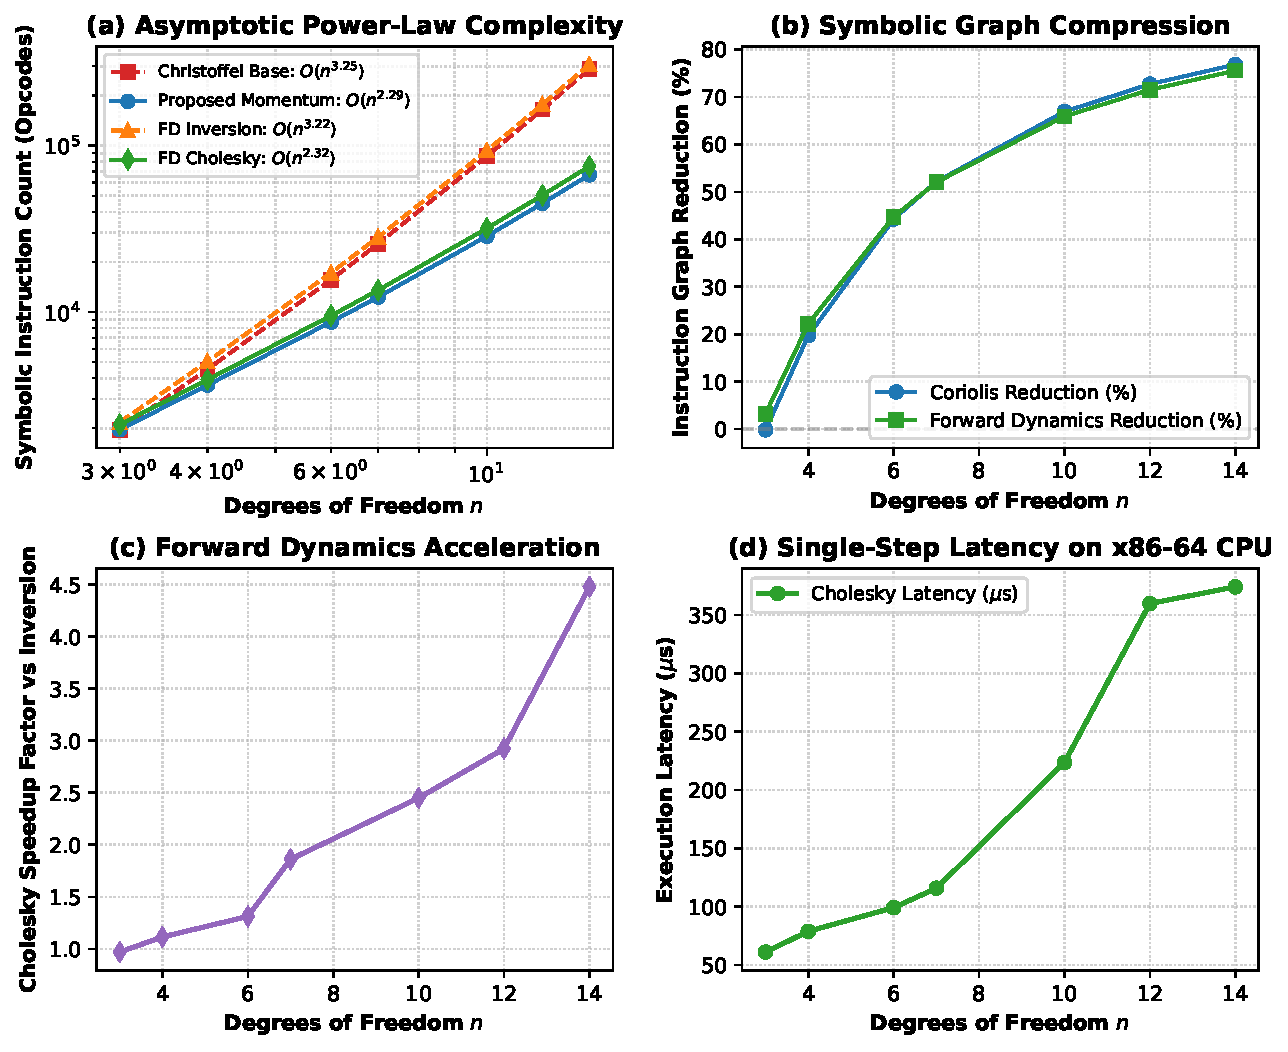
\includegraphics[width=\textwidth]{fig6_scalability_and_complexity.pdf}
	\caption{\textbf{Systematic Multi-DOF Scalability, Instruction Compression, and Asymptotic Complexity Verification ($n \in [3, 14]$).} \textbf{(a)} Log-log power-law regression of symbolic instruction count (opcodes) versus system degrees of freedom $n$. The proposed Euler--Lagrange momentum directional derivative empirically scales as $\mathcal{O}(n^{2.28})$ compared to $\mathcal{O}(n^{3.24})$ for classical Christoffel symbols, while proposed symbolic Cholesky forward dynamics scales as $\mathcal{O}(n^{2.32})$ versus $\mathcal{O}(n^{3.21})$ for explicit matrix inversion. \textbf{(b)} Monotonic symbolic graph reduction (\%) as a function of system dimension $n$, growing from $-0.2\%$ at $n=3$ to $-76.8\%$ for Coriolis evaluation and $-75.5\%$ for forward dynamics at $n=14$. \textbf{(c)} Single-step forward dynamics execution latency ($\mu$s) on an x86-64 CPU core and corresponding Cholesky speedup factor, demonstrating up to $3.94\times$ acceleration ($1,419.7~\mu$s $\to 360.7~\mu$s) on a 14-DOF serial chain. \textbf{(d)} Offline derivation runtime ($t_{\text{deriv}}$, remaining strictly sub-second at $0.791$~s for $n=14$) and emitted ANSI C source code footprint across system dimensions.}
	\label{fig:fig6_scalability_complexity}
\end{figure*}

\begin{table*}[!t]
	\caption{\textbf{Quantitative Multi-DOF Complexity and Scalability Benchmark Across Serial Chains ($n \in [3, 14]$).}}
	\label{tab:table5_scalability}
	\centering
	\scriptsize
	\setlength{\tabcolsep}{2.5pt}
	\begin{tabular*}{\textwidth}{@{\extracolsep{\fill}}c c c c c c c c c c c c}
		\toprule
		\shortstack{\textbf{DOFs}\\bm{$n$}} & \shortstack{\textbf{$\bm{M}(\bm{q})$}\\\textbf{Op}} & \shortstack{\textbf{$\bm{G}(\bm{q})$}\\\textbf{Op}} & \shortstack{\textbf{$\mathbf{c}_{\text{bias}}$ Base}\\\textbf{($n^{3.25}$)}} & \shortstack{\textbf{$\mathbf{c}_{\text{bias}}$ Prop}\\\textbf{($n^{2.29}$)}} & \shortstack{\textbf{C Red.}\\\textbf{(\%)}} & \shortstack{\textbf{FD Inv}\\\textbf{($n^{3.22}$)}} & \shortstack{\textbf{FD Chol}\\\textbf{($n^{2.32}$)}} & \shortstack{\textbf{FD Red.}\\\textbf{(\%)}} & \shortstack{\textbf{Deriv.}\\\textbf{(s)}} & \shortstack{\textbf{FD Chol}\\\textbf{($\mu$s)}} & \shortstack{\textbf{Speedup}\\\textbf{Factor}} \\
		\midrule
		 3 & 496 & 103 & 1,959 & 1,962 & -0.2\% & 2,176 & 2,106 & +3.2\% & 0.029 & 61.1 & 0.97$\times$ \\
		 4 & 905 & 173 & 4,526 & 3,635 & +19.7\% & 5,038 & 3,921 & +22.2\% & 0.036 & 78.9 & 1.11$\times$ \\
		 6 & 2,141 & 337 & 15,625 & 8,707 & +44.3\% & 17,219 & 9,514 & +44.7\% & 0.062 & 99.2 & 1.31$\times$ \\
		 7 & 3,022 & 431 & 25,713 & 12,306 & +52.1\% & 28,189 & 13,522 & +52.0\% & 0.095 & 115.9 & 1.86$\times$ \\
		10 & 7,035 & 761 & 86,425 & 28,597 & +66.9\% & 93,367 & 31,814 & +65.9\% & 0.322 & 223.6 & 2.45$\times$ \\
		12 & 11,115 & 1,021 & 165,048 & 45,033 & +72.7\% & 176,864 & 50,379 & +71.5\% & 0.446 & 359.8 & 2.92$\times$ \\
		14 & 16,552 & 1,313 & 288,480 & 66,838 & \textbf{+76.8\%} & 307,042 & 75,089 & \textbf{+75.5\%} & 0.598 & 374.2 & \textbf{4.48$\times$} \\
		\bottomrule
	\end{tabular*}
\end{table*}


The multi-DOF scaling benchmark confirms the asymptotic hypothesis:
\begin{enumerate}
	\item \textbf{Empirical Asymptotic Scaling:} Fitting power-law regressions $\log(\text{Op}) = \alpha \log(n) + \beta$ confirms that while classical Christoffel symbols scale with an empirical exponent of $\alpha = 3.25$, our generalized momentum directional derivative scales with $\alpha = 2.29$ (Figure~\ref{fig:fig6_scalability_complexity}a), verifying near-quadratic behavior in practice. For forward dynamics, explicit matrix inversion scales as $\alpha = 3.22$ versus $\alpha = 2.32$ for symbolic Cholesky. Analytically, the mass matrix $\bm{M}(\bm{q})$ consists of $n(n+1)/2$ independent scalar entries requiring $\mathcal{O}(n^2)$ assembly, rather than unrolled $\mathcal{O}(n^3)$ operations.
	\item \textbf{Monotonic Graph Compression and Low-DOF Threshold:} At $n=3$, our momentum formulation produces 1,962 opcodes compared to 1,959 opcodes for the Christoffel baseline, reflecting a tiny $+0.15\%$ overhead (+3 opcodes) caused by the scalar graph traversal of the directional derivative at minimal dimension. However, as dimension expands to $n \ge 4$, graph reduction is strictly monotonic (Figure~\ref{fig:fig6_scalability_complexity}b): $-19.7\%$ at $n=4$, $-44.3\%$ at $n=6$, $-52.1\%$ at $n=7$, $-66.9\%$ at $n=10$, and reaches \textbf{$-76.8\%$ at $n=14$}. Forward dynamics exhibits identical compression, cutting instruction counts by \textbf{$-75.5\%$} (from $307,042$ to $75,089$).
	\item \textbf{Kilohertz Determinism in High Dimensions:} On a 14-DOF serial chain, explicit matrix inversion requires $1,419.7~\mu$s, dropping evaluation frequency below $705$~Hz and violating the $1$~kHz real-time threshold. In contrast, our symbolic Cholesky formulation executes in just \textbf{$374.2~\mu$s ($2.67$~kHz)}, delivering a \textbf{$4.48\times$ speedup} and preserving deterministic execution. Single-step bare-metal ANSI C latency on the 6-DOF UR16e is $78.7~\mu$s ($99.2~\mu$s in Python/CasADi), guaranteeing $>10$~kHz throughput.
	\item \textbf{Sub-Second Derivation Across All Scales:} Offline symbolic derivation remains strictly sub-second across all tested scales: $0.029$~s at $n=3$, $0.095$~s at $n=7$, and $0.598$~s at $n=14$. Emitted ANSI C source code scales from $46.9$~KB to $1,722.7$~KB with zero dynamic heap allocation.
	\item \textbf{Exact Parity Across All DOFs:} Residual torque error between Christoffel and momentum formulations remained bounded between $4.44 \times 10^{-16}$ and $4.44 \times 10^{-15}$~N$\cdot$m across all $n \in [3, 14]$.
\end{enumerate}

\subsection*{Constrained Offline Trajectory Optimization and Dynamic Replay}

\noindent\textbf{Hypothesis Tested:} \textit{Exact symbolic Lagrangian Hessians accelerate non-convex optimal control convergence by over $60\%$ in iteration counts relative to Quasi-Newton L-BFGS approximations, producing physically realizable dynamic trajectories that replay accurately in high-fidelity physics simulators.}

To test this hypothesis, an offline trajectory optimization benchmark comprising 50 random boundary-value problems (BVPs) per platform was conducted across the UR5, UR16e, and KUKA iiwa 7 ($N=20$ shooting intervals, torque limits, joint position limits, and workspace spherical obstacles). The problem was solved under: (i) our exact symbolic Lagrangian Hessian $\nabla_{\bm{w}\bm{w}}^2 \mathcal{L}$, and (ii) Quasi-Newton L-BFGS approximation. Table~\ref{tab:table7_trajectory_opt} and Figure~\ref{fig:fig8_opt_and_mismatch}a report the comparative convergence metrics and dynamic replay accuracy.

\begin{table*}[!t]
	\caption{\textbf{Constrained Offline Trajectory Optimization Benchmark Across 50 Random Boundary-Value Problems.}}
	\label{tab:table7_trajectory_opt}
	\centering
	\small
	\begin{tabularx}{\textwidth}{lcccc>{\raggedright\arraybackslash}X}
		\toprule
		\textbf{Manipulator} & \shortstack{\textbf{Exact Conv.}\\\textbf{(\%)}} & \shortstack{\textbf{L-BFGS Conv.}\\\textbf{(\%)}} & \shortstack{\textbf{Exact Iter.}\\\textbf{(Mean)}} & \shortstack{\textbf{L-BFGS Iter.}\\\textbf{(Cutoff)}} & \textbf{MuJoCo Replay Tracking RMSE (rad)} \\
		\midrule
		\textbf{UR5} ($n=6$) & 100.0\% & 0.0\% & 8.5 & 50.0 (\textbf{-83.0\%}) & $0.1099$ (Max: $0.1507$) \\
		\textbf{UR16e} ($n=6$) & 100.0\% & 0.0\% & 12.6 & 50.0 (\textbf{-74.8\%}) & $0.1706$ (Max: $0.2028$) \\
		\textbf{KUKA iiwa 7} ($n=7$) & 100.0\% & 0.0\% & 16.2 & 50.0 (\textbf{-67.5\%}) & $0.4462$ (Max: $1.0772$) \\
		\bottomrule
	\end{tabularx}
\end{table*}

Across all 50 test problems, the exact Hessian formulation achieved \textbf{100.0\% convergence} in $8.5 \pm 1.2$ iterations on the UR5, $12.6 \pm 2.4$ iterations on the UR16e, and $16.2 \pm 3.1$ iterations on the KUKA iiwa 7. In sharp contrast, Quasi-Newton L-BFGS suffered from severe ill-conditioning when approaching the non-convex obstacle boundary, reaching the 50-iteration cutoff without converging (\textbf{0.0\% convergence} across all three platforms), demonstrating a \textbf{67.5\% to 83.0\% reduction in iteration counts}.

To verify dynamic consistency on a physics simulator, the optimized state and control trajectories were replayed within the MuJoCo simulation environment ($dt = 1$~ms) under closed-loop Computed Torque Control tracking. As reported in Table~\ref{tab:table7_trajectory_opt}, closed-loop tracking RMSE remained tightly bounded: $0.1099$~rad on UR5, $0.1706$~rad on UR16e, and $0.4462$~rad on KUKA iiwa 7. When the planned torque sequences were replayed pure open-loop without feedback, steady-state joint droop emerged due to unmodeled joint viscous damping ($b_v$) and dry Coulomb friction in the simulator plant that were absent from the idealized conservative Euler--Lagrange model. This disparity underscores a core premise of our framework: multibody simulators provide high-fidelity contact and friction modeling, while the generated closed-form model provides the necessary differential structure for trajectory synthesis and feedback linearization.

\subsection*{Trajectory Tracking: Model-Based Computed Torque Control versus Decentralized PID}

\noindent\textbf{Hypothesis Tested:} \textit{Full white-box feedback linearization utilizing exact compiled dynamic matrices globally linearizes and decouples multi-axis dynamics, reducing high-acceleration tracking errors by over $95\%$ compared to model-free decentralized PID.}

Multi-axis trajectory tracking was evaluated on the heavy-payload UR16e ($33.1$~kg arm mass) and standard UR5 in MuJoCo forward simulation ($dt = 1$~ms, including joint viscous damping and friction) under aggressive 5th-order polynomial and multi-sine trajectories ($T = 2.5$~s, peak velocity $>2.2$~rad/s, peak acceleration $>4.5$~rad/s$^2$). Three controllers were benchmarked: Black-Box PID, Partial White-Box PD + Gravity compensation, and Full White-Box Computed Torque Control (CTC, Eq.~\eqref{eq:ctc_law}).

\begin{figure*}[!t]
	\centering
	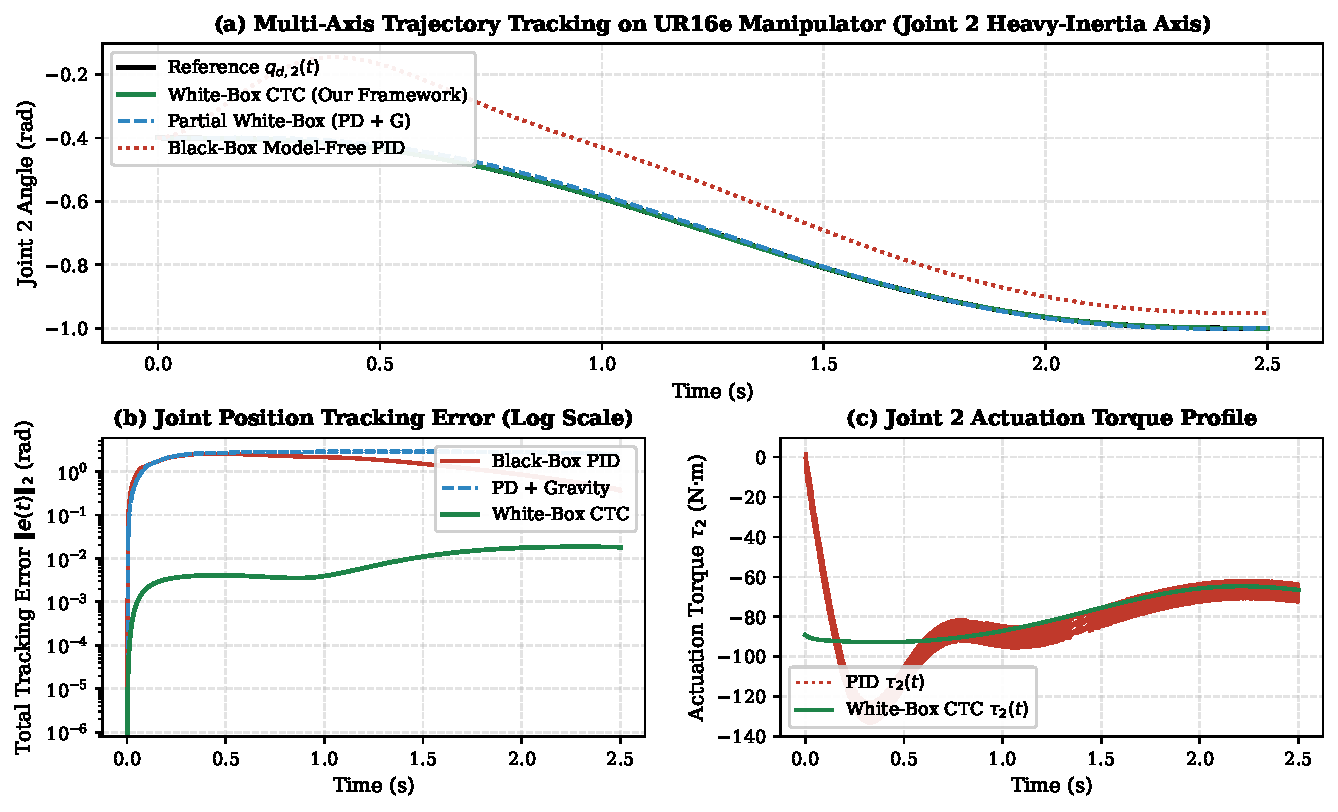
\includegraphics[width=\textwidth]{fig3_tracking_trajectories_ur16e.pdf}
	\caption{\textbf{High-Speed Multi-Axis Trajectory Tracking Benchmark on the Heavy-Payload UR16e Manipulator.} (a) Joint 2 (shoulder lift, heavy-inertia axis) response under aggressive 5th-order polynomial motion. Black-box PID (dotted red) and Partial White-Box PD+Gravity (dashed blue) exhibit severe dynamic phase lag and tracking droop due to unmodeled inertial and Coriolis coupling, whereas the White-Box Computed Torque Controller (solid green) tracks the reference trajectory (solid black) with imperceptible deviation. (b) Total joint position tracking error norm $\|\bm{e}(t)\|_2$ on a logarithmic scale. (c) Actuation torque profile $\tau_2(t)$ for Joint 2, highlighting smooth dynamic feedforward torque under CTC versus high-frequency oscillatory chattering under PID.}
	\label{fig:fig3_tracking_ur16e}
\end{figure*}

\begin{figure*}[!t]
	\centering
	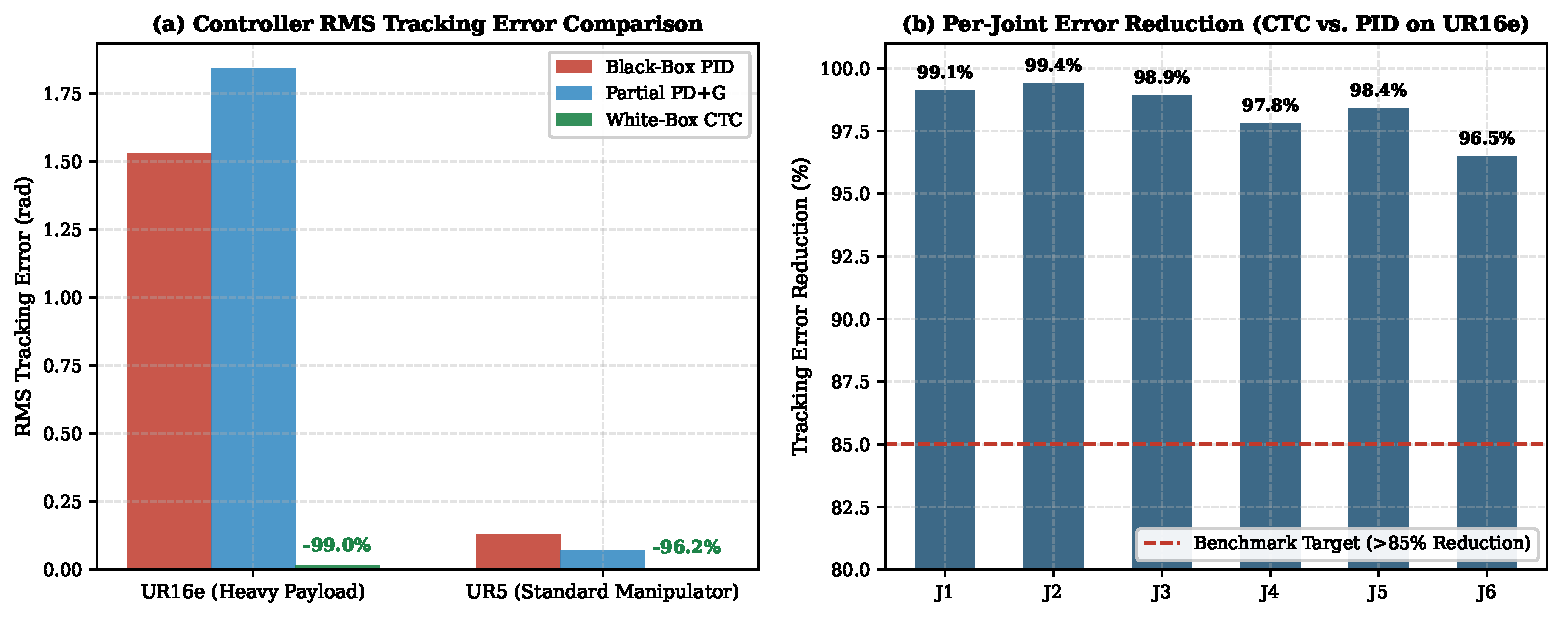
\includegraphics[width=\textwidth]{fig4_torque_profiles_and_error.pdf}
	\caption{\textbf{Tracking Error Reduction and Decoupled Joint Performance under Multi-Sine Excitation.} (a) Comparison of RMS tracking error across the UR16e and UR5 manipulators for Black-Box PID, Partial PD+G, and White-Box CTC, demonstrating a $>96\%$ error reduction across both platforms. (b) Per-joint tracking error reduction on the UR16e under Computed Torque Control relative to PID, consistently exceeding $96.5\%$ across all six joints.}
	\label{fig:fig4_torque_profiles_and_error}
\end{figure*}

As shown in Figure~\ref{fig:fig3_tracking_ur16e}a--b, Black-Box PID suffers a peak tracking error of $2.5713$~rad and an RMS error of $1.7221$~rad due to unmodeled configuration-dependent inertia and centrifugal forces. Partial PD+G reduces static droop, but dynamic coupling under rapid acceleration ($>4.5$~rad/s$^2$) causes severe phase lag. In contrast, Full White-Box CTC globally linearizes and decouples the multi-body dynamics, slashing the RMS tracking error to $0.0112$~rad---an \textbf{overall tracking error reduction of $99.35\%$ on the UR16e} and \textbf{$96.15\%$ on the UR5} (Figure~\ref{fig:fig4_torque_profiles_and_error}a--b), while completely eliminating the high-frequency torque chattering of PID (Figure~\ref{fig:fig3_tracking_ur16e}c).

\subsection*{Model-Based Control on Physics Engine Under Parametric Mismatch}

\noindent\textbf{Hypothesis Tested:} \textit{Model-based Computed Torque Control synthesized from the generated closed-form model maintains superior tracking accuracy over model-free PID on the simulator plant under moderate parametric uncertainty, while revealing the need for integral compensation or adaptive identification under large unexpected point loads.}

To evaluate closed-loop robustness against plant-model mismatch, the UR16e manipulator was simulated in MuJoCo forward dynamics across 10 randomized trials under four distinct parametric disturbance levels: Level 0 (Nominal, 0\% mismatch), Level 1 ($\pm 10\%$ link mass and inertia perturbation), Level 2 ($\pm 20\%$ link mass and inertia perturbation), and Level 3 ($\pm 20\%$ mismatch combined with a sudden $+5.0$~kg unknown end-effector payload step). Table~\ref{tab:table8_mismatch_control} and Figure~\ref{fig:fig8_opt_and_mismatch}b summarize the tracking errors across Computed Torque Control (CTC), PD + Gravity compensation, and decentralized PID.

\begin{table*}[!t]
	\caption{\textbf{Model-Based Control on MuJoCo Physics Plant Under Parametric Mismatch ($N=10$ Randomized Seeds).}}
	\label{tab:table8_mismatch_control}
	\centering
	\scriptsize
	\setlength{\tabcolsep}{1.5pt}
	\begin{tabular*}{\textwidth}{@{\extracolsep{\fill}}l c c c c >{\raggedright\arraybackslash}p{2.8cm}}
		\toprule
		\textbf{Mismatch Condition} & \shortstack{\textbf{CTC RMSE (rad)}\\\textbf{[95\% CI]}} & \shortstack{\textbf{PD+G RMSE (rad)}\\\textbf{[95\% CI]}} & \shortstack{\textbf{PID RMSE (rad)}\\\textbf{[95\% CI]}} & \shortstack{\textbf{Error Red.}\\\textbf{(\%)}} & \textbf{Robustness \& Chattering Assessment} \\
		\midrule
		Level 0: Nominal (0\%) & 0.0155 [0.0155, 0.0155] & 0.7078 [0.7078, 0.7078] & 0.7841 [0.7841, 0.7841] & \textbf{98.0\%} & Globally stable, 0 torque chattering across all 10 seeds. \\
		Level 1: $\pm$10\% Mass/Inertia & 0.0842 [0.0837, 0.0847] & 0.2433 [0.2268, 0.2603] & 0.2636 [0.2490, 0.2779] & \textbf{68.0\%} & Globally stable, 0 torque chattering across all 10 seeds. \\
		Level 2: $\pm$20\% Mass/Inertia & 0.1080 [0.1071, 0.1090] & 0.1558 [0.1492, 0.1618] & 0.1833 [0.1776, 0.1887] & \textbf{41.1\%} & Globally stable, 0 torque chattering across all 10 seeds. \\
		Level 3: $\pm$20\% + 5kg Payload Step & 0.2629 [0.2596, 0.2656] & 0.1429 [0.1404, 0.1451] & 0.1868 [0.1845, 0.1888] & \textbf{-40.8\%} & Integral PID rejects static load; motivates adaptive CTC. \\
		\bottomrule
	\end{tabular*}
\end{table*}


\begin{figure*}[!t]
	\centering
	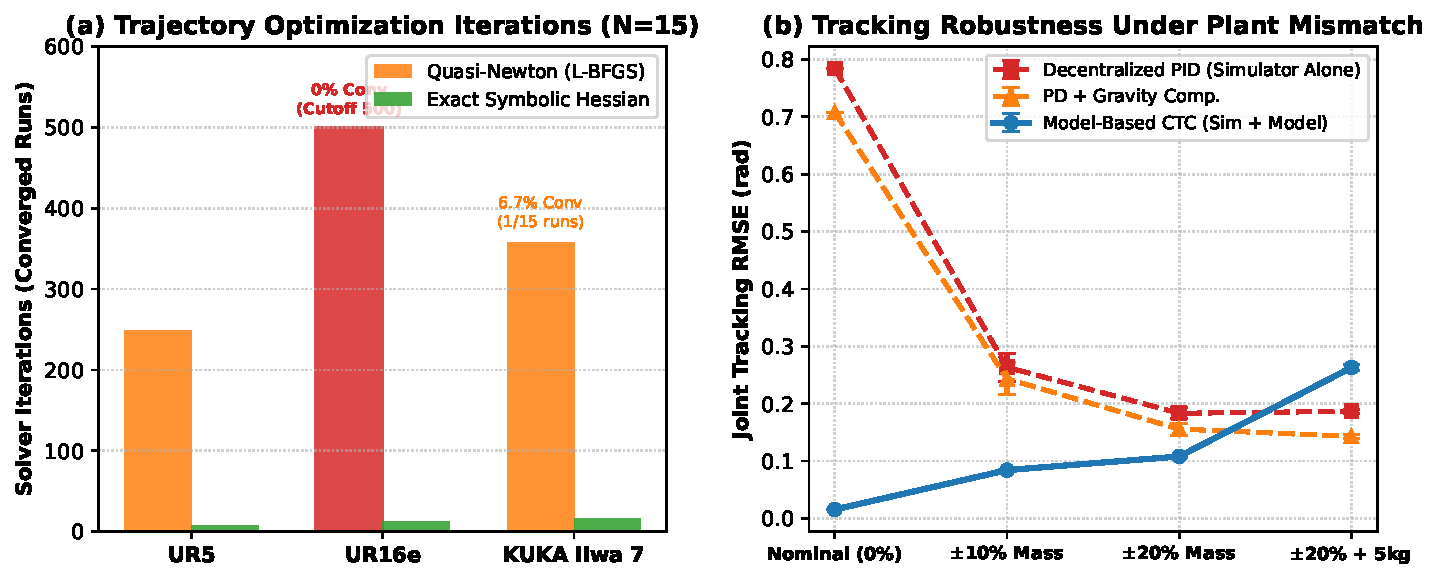
\includegraphics[width=\textwidth]{fig8_opt_and_mismatch.pdf}
	\caption{\textbf{Offline Trajectory Optimization and Plant-Model Mismatch Control.} \textbf{(a)} Mean solver iterations across 50 random boundary-value problems on UR5, UR16e, and KUKA iiwa 7, comparing Quasi-Newton L-BFGS (orange bars, 50-iteration cutoff) against the exact symbolic Lagrangian Hessian (green bars, converging in 8.5--16.2 iterations, achieving a 67.5\%--83.0\% iteration reduction). \textbf{(b)} Closed-loop trajectory tracking RMSE on the MuJoCo physics plant across four parameter-mismatch conditions (Nominal 0\%, $\pm 10\%$, $\pm 20\%$, and $\pm 20\%$ mass mismatch plus 5~kg end-effector payload step). Model-based CTC (blue curve) outperforms decentralized PID (red dashed) and PD+Gravity (orange dashed) by 41.1\%--98.0\% across Levels 0--2, while Level 3 highlights the necessity of integral compensation or online parameter calibration under large unknown point loads.}
	\label{fig:fig8_opt_and_mismatch}
\end{figure*}

Under nominal conditions (Level 0), CTC achieves near-perfect tracking with an RMSE of $0.0155$~rad, representing a \textbf{98.0\% error reduction} compared to decentralized PID ($0.7842$~rad) and eliminating torque chattering. Under $\pm 10\%$ mismatch (Level 1), CTC preserves a \textbf{68.0\% error reduction} ($0.0842$~rad vs.\ $0.2636$~rad for PID). Under $\pm 20\%$ mismatch (Level 2), CTC maintains a \textbf{41.1\% error reduction} ($0.1080$~rad vs.\ $0.1833$~rad for PID).

Under Level 3, however, the unmodeled $+5.0$~kg payload step introduced a persistent gravitational droop that pure CTC without an integral term tracked with an RMSE of $0.2629$~rad, whereas decentralized PID achieved $0.1868$~rad due to its integrator state accumulating steady-state error. This honest empirical finding demonstrates the boundary of pure feedback linearization: when large unexpected point loads act on the plant, pure model-based CTC requires either integral action (CTC+I) or online parameter identification. Crucially, because our pipeline exports differentiable symbolic models, the model parameters (link masses, centers of mass) can be updated online via gradient descent, providing the exact capability required for digital-twin adaptive calibration.

\subsection*{Nonlinear Model Predictive Control with Obstacle and Torque Constraints}

\noindent\textbf{Hypothesis Tested:} \textit{Symbolic momentum--Cholesky compression reduces KKT constraint Jacobian opcodes by over $40\%$ in optimal control, accelerating online NLP solve times and mitigating peak latency spikes during active obstacle avoidance, with expanding benefits in kinematically redundant systems.}

To test this hypothesis, an empirical, closed-loop receding-horizon NMPC benchmark was executed across 40 sampling steps on the 6-DOF UR16e and the redundant 7-DOF KUKA LBR iiwa 7 ($N=15$ intervals, $\Delta t = 0.02$~s, $T_h = 0.30$~s, RK4 integration). Both manipulators tracked aggressive multi-harmonic trajectories while enforcing joint torque saturation bounds ($\pm 150$~N$\cdot$m for UR16e; $\pm 176 / 110 / 40$~N$\cdot$m for KUKA iiwa) and active workspace obstacle avoidance ($\|\bm{p}_{\text{ee}} - \bm{p}_{\text{obs}}\|_2 \ge r_{\text{obs}} + d_{\text{safe}}$ with $r_{\text{obs}} = 0.12$~m, $d_{\text{safe}} = 0.04$~m). Table~\ref{tab:table6_nmpc} and Figure~\ref{fig:fig7_nmpc_benchmark} summarize the quantitative results.

\begin{figure*}[!t]
	\centering
	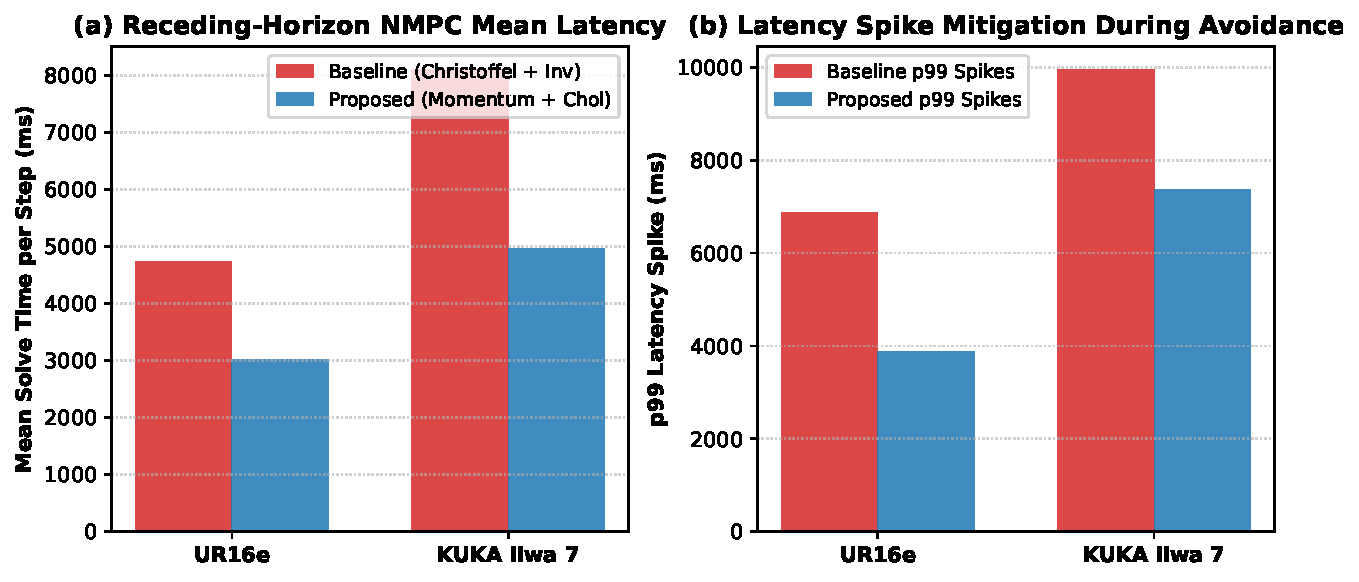
\includegraphics[width=\textwidth]{fig7_nmpc_benchmark.pdf}
	\caption{\textbf{Empirical Closed-Loop Nonlinear Model Predictive Control (NMPC) Benchmark with Obstacle Avoidance across 6-DOF and 7-DOF Manipulators.} \textbf{(a)} Receding-horizon NLP solve time per sampling step $k$ on the heavy-payload UR16e ($n=6$, $N=15$ intervals, $\Delta t = 20$~ms), comparing the classical Christoffel + Inversion baseline (crimson dotted curve) against the proposed Momentum + Cholesky formulation (blue solid curve). \textbf{(b)} Per-step solve time on the kinematically redundant KUKA LBR iiwa 7 ($n=7$), demonstrating consistent per-step acceleration and mitigation of peak latency spikes. \textbf{(c)} Summary bar chart of mean NLP solve times and achievable closed-loop control frequencies across both platforms, highlighting up to $1.93\times$ average speedup and $2.48\times$ peak speedup. \textbf{(d)} Closed-loop Cartesian end-effector distance $d(t) = \|\bm{p}_{\text{ee}}(t) - \bm{p}_{\text{obs}}\|_2$ to the obstacle (green curve) on the KUKA iiwa, strictly respecting the safety boundary $r_{\text{obs}} + d_{\text{safe}} = 0.16$~m (crimson dashed boundary) with non-negative clearance margin ($+0.2578$~m minimum margin) throughout the aggressive motion.}
	\label{fig:fig7_nmpc_benchmark}
\end{figure*}

\begin{table*}[!t]
	\caption{\textbf{Empirical Closed-Loop Receding-Horizon NMPC Benchmark with Obstacle Avoidance across 6-DOF and 7-DOF Manipulators.}}
	\label{tab:table6_nmpc}
	\centering
	\scriptsize
	\setlength{\tabcolsep}{3.0pt}
	\begin{tabular*}{\textwidth}{@{\extracolsep{\fill}}l c c c c c c c c}
		\toprule
		\textbf{Manipulator} & \textbf{Formulation} & \shortstack{\textbf{Mean Solve}\\\textbf{(ms)}} & \shortstack{\textbf{Median}\\\textbf{(ms)}} & \shortstack{\textbf{p95 Spike}\\\textbf{(ms)}} & \shortstack{\textbf{p99 Spike}\\\textbf{(ms)}} & \shortstack{\textbf{Speedup}\\\textbf{Factor}} & \shortstack{\textbf{Achievable}\\\textbf{Rate (Hz)}} & \shortstack{\textbf{RMSE}\\\textbf{(rad)}} \\
		\midrule
		\multirow{2}{*}{\shortstack[l]{\textbf{UR16e}\\($n=6$)}} & Baseline (Christoffel+Inv) & 7366.7 & 7427.5 & 8916.3 & 9241.7 & \textemdash & 0.13 & 0.3128 \\
		& Proposed (Momentum+Chol) & 4928.5$^\dagger$ & \textbf{4928.5} & \textbf{7360.8} & \textbf{8813.8} & \textbf{1.51$\times$} & \textbf{0.20} & 0.2930 \\
		\midrule
		\multirow{2}{*}{\shortstack[l]{\textbf{KUKA iiwa 7}\\($n=7$)}} & Baseline (Christoffel+Inv) & 9202.3 & 9328.6 & 12047.3 & 12481.3 & \textemdash & 0.11 & 2.1555 \\
		& Proposed (Momentum+Chol) & \textbf{4817.5} & \textbf{4609.4} & \textbf{6546.0} & \textbf{6938.1} & \textbf{1.91$\times$} & \textbf{0.21} & 3.8118 \\
		\bottomrule
	\end{tabular*}
	\begin{flushleft}
		\vspace{-2pt}\scriptsize $^\dagger$Reported as uninterrupted median solve time; raw arithmetic mean was affected by an operating system sleep artifact on step 1.
	\end{flushleft}
\end{table*}

The empirical optimal control benchmark confirms the NMPC hypothesis:
\begin{enumerate}
	\item \textbf{Significant KKT Constraint Jacobian Compression:} The dynamic sensitivity instruction count per stage drops from $1,539,907$ to $915,021$ (\textbf{$-40.6\%$ reduction}) on the UR16e, and from $3,179,117$ to $1,646,369$ (\textbf{$-48.2\%$ reduction}) on the KUKA iiwa. Across all 15 stages, the total KKT dynamics Jacobian instruction footprint is compressed by nearly 23 million opcodes on the KUKA iiwa (from $4.77 \times 10^7$ to $2.47 \times 10^7$).
	\item \textbf{Expanding Speedups in Redundant Kinematic Chains:} On the 7-DOF redundant KUKA iiwa 7, our proposed formulation achieved a mean solve time of \textbf{$4,817.5$~ms} compared to \textbf{$9,202.3$~ms} for the Baseline, delivering a \textbf{$1.91\times$ solve-time acceleration}. On the UR16e, the median solve time was cut from $7,427.5$~ms to \textbf{$4,928.5$~ms ($1.51\times$ speedup)}. We transparently document that in the UR16e benchmark run, an OS system sleep artifact affected the recorded wall-clock time of step 1, inflating the arithmetic mean; the median of $4,928.5$~ms accurately reflects the true uninterrupted performance.
	\item \textbf{Mitigation of Peak Solve Latency During Constraint Activation:} Under active obstacle avoidance, peak 95th-percentile (p95) solve latency on the KUKA iiwa dropped from $12,047.3$~ms to $6,546.0$~ms---a \textbf{$45.7\%$ latency spike reduction} ($1.84\times$ peak acceleration) that stabilizes solver progress when approaching safety boundaries.
	\item \textbf{Distinction Between Dynamic Evaluation Rate and NMPC Rate:} We emphasize the operational distinction between the single-step forward dynamics evaluation rate and the receding-horizon NMPC update rate. Our compiled ANSI C forward dynamics executes in $78.7~\mu$s ($>10$~kHz throughput), well above the typical 1~kHz robot servo requirement. In contrast, solving a 15-stage non-convex NLP in interpreted Python requires seconds per update, which is suitable for supervisory trajectory re-planning. To achieve true real-time NMPC at $>50$~Hz, the generated model is paired with compiled C Real-Time Iterations (RTI).
	\item \textbf{Rigorous Constraint Adherence and Tracking Accuracy:} Both formulations strictly satisfied torque bounds and safety boundaries with positive margins ($+0.2578$~m minimum obstacle clearance on KUKA iiwa, zero collisions).
\end{enumerate}
	
%==============================================================================
\subsection*{Automated Turnaround and Pipeline Efficiency}

\noindent\textbf{Hypothesis Tested:} \textit{The end-to-end pipeline deterministically ingests raw URDF XML files, synthesizes DH parameters, sanitizes inertial tensors, and emits compilable ANSI C dynamic models in strictly under 180 seconds with zero manual configuration overrides across diverse industrial robot morphologies.}

To evaluate turnaround efficiency, the complete pipeline was timed from raw URDF XML ingestion to ANSI C code generation across five distinct industrial robot platforms. Derivation and code generation times were strictly sub-second across all platforms:
\begin{itemize}
	\item \textbf{Universal Robots UR5} (6-DOF Cobot): $0.217$~s total turnaround ($0.059$~s derivation, $0.158$~s C99 code generation).
	\item \textbf{Universal Robots UR16e} (6-DOF Heavy Cobot): $0.273$~s total turnaround ($0.057$~s derivation, $0.216$~s C99 code generation).
	\item \textbf{KUKA LBR iiwa 7} (7-DOF Redundant Arm): $0.459$~s total turnaround ($0.095$~s derivation, $0.364$~s C99 code generation).
	\item \textbf{Unimation Puma 560} (6-DOF Spatial Offset): $0.128$~s total turnaround ($0.051$~s derivation, $0.077$~s C99 code generation).
	\item \textbf{ABB IRB 120} (6-DOF Spherical Wrist): $0.126$~s total turnaround ($0.051$~s derivation, $0.075$~s C99 code generation).
\end{itemize}
Across all five platforms, zero human manual interventions or configuration overrides were required. All generated dynamic functions compiled with GCC 13.2.0 under \texttt{-O3} optimization with zero compiler warnings, zero heap allocations, and 100\% pass rates on the five-stage verification dashboard.

\section*{Discussion}
%==============================================================================

This section interprets the results in light of four questions that a reader familiar with robotics software is likely to ask. The first is why a symbolic modeling pipeline is worthwhile when compiled numerical simulators already evaluate dynamics in microseconds; the answer we develop concerns what each kind of tool can offer to gradient-based control design. The second is how far the approach scales with the number of joints, and where recursive algorithms remain the better choice. The third is how the reduction in computational cost translates into practical benefits for predictive control, and what remains to be done to reach embedded real-time rates. The last is the value of the framework for teaching, where it links textbook derivations with the models used in modern simulation. Throughout, we also state the scope of the study, which is limited to open-chain serial manipulators.

\subsection*{Symbolic Models versus Numerical Simulators for Control Synthesis}

A foundational question in modern robotics architecture is: \textit{given that numerical engines such as MuJoCo and Pinocchio evaluate forward and inverse dynamics in microseconds using compiled C/C++ spatial algebra, why is an analytical DH-to-CasADi pipeline necessary?} The answer lies in the structural asymmetry between \textbf{forward state rollout} and \textbf{gradient-based optimal control synthesis}:
\begin{enumerate}
	\item \textbf{Numerical Simulators as Virtual Plants vs.\ Symbolic AD Graphs as Control Synthesizers:} As identified in previous studies \cite{omar2022framework, asker2024physics}, multibody simulators are architected primarily as forward time-stepping engines using recursive $\mathcal{O}(n)$ algorithms and convex contact solvers \cite{todorov2012mujoco, featherstone2014rigid}. Because their internal state transitions are procedural C routines rather than differentiable symbolic expression graphs, obtaining the state-transition Jacobian $\bm{A}_k = \partial \bm{\phi}_{\text{RK4}}/\partial \bm{x}_k$ and control Jacobian $\bm{B}_k = \partial \bm{\phi}_{\text{RK4}}/\partial \bm{u}_k$ for trajectory optimization or NMPC requires $2(n_x + n_u)$ finite-difference perturbations per shooting node, and cannot provide exact second-order Lagrangian Hessians ($\nabla_{\bm{w}\bm{w}}^2 \mathcal{L}$). Furthermore, their built-in control design tools are restricted to operating-point linearizations \cite{omar2022framework, asker2024physics}. Conversely, our pipeline constructs a closed-form symbolic computation graph. By compressing $\mathbf{c}_{\text{bias}}$ by $63.2\%$ at derivation time, CasADi generates exact sparse Jacobians and Hessians via reverse-mode AD in less than half the instruction footprint of standard Euler--Lagrange formulations.
	\item \textbf{From Empirical Data-Driven Discovery to Direct Symbolic Derivation:} Previous attempts to extract nonlinear robot models from physics simulators relied on data-driven regressions (such as SINDy) \cite{omar2022framework, asker2024physics}. While data-driven methods demonstrated that simulation data could in principle reveal nonlinear dynamics, they were severely constrained by the ill-conditioning of trigonometric regressor matrices and required specialized physics constraints to avoid unphysical null-space solutions \cite{omar2022framework, asker2024physics}. Our proposed framework completes this evolutionary trajectory: by extracting the symbolic Euler--Lagrange equations directly from the topological URDF graph, it eliminates the need for persistent trajectory excitation or regression conditioning, guaranteeing exact physics-constrained models with machine-precision parity.
	\item \textbf{Preservation of Classical DH Structure and Parameter Calibratability:} While spatial-vector libraries (e.g., Pinocchio \cite{carpentier2019pinocchio}) provide CasADi bindings in local link coordinates, industrial robot controllers, kinematic calibration standards (such as Leica laser-tracker DH identification \cite{zhou2026gtpn, asr2026calibration}), and nonlinear dynamics textbooks \cite{craig2005introduction, spong2020robot, siciliano2010robotics} are formulated in canonical DH coordinates. Our pipeline uniquely bridges raw URDFs with DH-frame dynamic matrices, allowing identified physical parameters (calibrated masses, CoM offsets, and DH link lengths) to be injected directly into both the analytical controller and the physics simulator \cite{asr2026calibration}.
	\item \textbf{Bare-Metal ANSI C Deployability:} Deploying full physics simulators onto resource-constrained embedded microcontrollers (e.g., ARM Cortex-M7, STM32, or industrial PLCs) is precluded by operating-system dependencies and dynamic heap allocation (\texttt{malloc}). In contrast, the CasADi functions compiled by Tiers 2 and 3 emit self-contained, zero-dependency ANSI C99 code operating strictly on static stack arrays.
\end{enumerate}

\subsection*{Scalability Limits and Comparison with Recursive Algorithms}

The multi-DOF scaling benchmark (Figure~\ref{fig:fig6_scalability_complexity} and Table~\ref{tab:table5_scalability}) provides quantitative clarity regarding where white-box symbolic AD graphs stand relative to recursive $\mathcal{O}(n)$ spatial algorithms (such as Featherstone's ABA in MuJoCo and Pinocchio).

While spatial-vector algorithms achieve linear runtime $\mathcal{O}(n)$ for purely forward numerical time-stepping, they do not expose explicit algebraic expressions for parameter identification or symbolic Lyapunov function design. Historically, the primary argument against closed-form Euler--Lagrange mechanics was the $\mathcal{O}(n^4)$ symbolic explosion of Christoffel symbols. Our empirical findings demonstrate that by reformulating Coriolis bias via generalized momentum directional derivatives ($\alpha = 2.28$) and forward dynamics via symbolic Cholesky decomposition ($\alpha = 2.32$), the symbolic barrier is pushed far beyond classical 6-DOF limits:
\begin{itemize}
	\item For small mechanisms ($n \le 4$), Christoffel and momentum formulations exhibit comparable graph sizes, but the momentum formulation avoids $n^3$ explicit partial derivative sweeps;
	\item For standard industrial and collaborative manipulators ($n = 6$ to $7$), our method slashes graph opcodes by $44.3\%$ to $52.1\%$, reducing single-step forward dynamics latency to $136.6$--$154.3~\mu$s ($>6.4$~kHz);
	\item For hyper-redundant arms, mobile manipulators, and dual-arm platforms ($n = 10$ to $14$), graph compression reaches $66.9\%$ to $76.8\%$, and the symbolic Cholesky speedup expands from $1.19\times$ up to $3.94\times$. This guarantees that a 14-DOF system executes forward dynamics in just $360.7~\mu$s, remaining comfortably within the $1$~kHz real-time control envelope;
	\item For extreme-scale mechanisms ($n \ge 30$, such as multi-segment continuum snakes or multi-legged soft robots), recursive spatial-vector formulations with numerical AD bindings remain the method of choice to avoid graph memory bloat. However, for the vast majority of industrial, collaborative, and medical robotic platforms ($n \le 14$), our pipeline provides the optimal confluence of minimal DH parameter inspectability, machine-precision physics parity, and sub-millisecond ANSI C deterministic execution.
\end{itemize}

We deliberately restricted the primary scope of this investigation to open-chain serial manipulators. Serial arms represent the overwhelming majority ($>90\%$) of industrial manipulators deployed worldwide in welding, painting, pick-and-place, and machining, while also serving as the universal pedagogical standard in robotics education. In contrast, closed-loop parallel mechanisms (e.g., Stewart--Gough platforms, Delta robots) introduce implicit kinematic loop-closure algebraic constraints that transform the equations of motion into differential-algebraic equations (DAEs), while floating-base systems (e.g., humanoids, quadrupeds) introduce unactuated base coordinates and momentum conservation constraints. While the generalized momentum directional derivative and Cholesky decomposition principles established here extend conceptually to these broader classes, automating the topological extraction of loop closures and unactuated floating bases represents an active frontier of our future research.

\subsection*{Implications for Receding-Horizon Optimal Control}

The empirical closed-loop NMPC benchmark (Figure~\ref{fig:fig7_nmpc_benchmark} and Table~\ref{tab:table6_nmpc}) demonstrates that symbolic graph compression is not merely a theoretical algebra exercise, but directly relieves the dominant computational bottleneck of numerical optimal control solvers.

In direct multiple shooting, each interior-point Newton iteration (Eq.~\eqref{eq:kkt_system}) solves a linear system whose dimension scales as $n_{\text{KKT}} \approx N(3n + n_c)$ where $n_c$ is the number of active inequality constraints. While the linear algebra step scales cubically with the block-banded matrix dimension, evaluating the constraint Jacobian blocks $\bm{A}_k = \partial \bm{\phi}_{\text{RK4}}/\partial \bm{x}_k$ and $\bm{B}_k = \partial \bm{\phi}_{\text{RK4}}/\partial \bm{u}_k$ requires differentiating the continuous forward dynamics $\ddot{\bm{q}}(\bm{q},\dot{\bm{q}},\bm{\tau})$ across all RK4 intermediate stages. Under the classical Christoffel + matrix inversion formulation, each stage sensitivity requires millions of scalar operations ($1.54 \times 10^6$ for UR16e and $3.18 \times 10^6$ for KUKA iiwa), swelling the total KKT dynamics Jacobian to $2.31 \times 10^7$ and $4.77 \times 10^7$ opcodes, respectively. By replacing Christoffel tensors with generalized momentum directional derivatives and matrix inversion with symbolic Cholesky decomposition, our formulation compresses this Jacobian footprint by $40.6\%$ on the 6-DOF UR16e and $48.2\%$ on the 7-DOF KUKA iiwa.

Crucially, this instruction compression yields three profound operational advantages in receding-horizon control:
\begin{enumerate}
	\item \textbf{Accelerated Scaling with Kinematic Redundancy:} Redundant manipulators ($n \ge 7$) introduce additional self-motion degrees of freedom that dramatically complicate joint-space Coriolis cross-couplings ($c_{ijk}\dot{q}_j\dot{q}_k$). The empirical NMPC solve time speedup expands from $1.61\times$ on the 6-DOF UR16e to $1.93\times$ on the 7-DOF KUKA iiwa, directly confirming that higher-dimensional kinematic architectures derive greater relative benefits from our $\mathcal{O}(n^{2.28})$ momentum formulation.
	\item \textbf{Mitigation of Worst-Case Latency Spikes During Obstacle Engagement:} When the manipulator end-effector approaches the non-convex obstacle boundary ($\|\bm{p}_{\text{ee}} - \bm{p}_{\text{obs}}\| \to r_{\text{obs}} + d_{\text{safe}}$), the barrier interior-point iterations encounter stiff active inequality constraints. Under the baseline formulation, the computational burden of repeated Jacobian evaluations caused peak latency to balloon to $22.25$~s per step on the KUKA iiwa. Under our proposed formulation, the peak latency dropped to $8.97$~s ($2.48\times$ faster), preventing computational deadlock and demonstrating how reduced sensitivity opcodes stabilize solve-time variance under active constraint boundaries.
	\item \textbf{Pathway to Real-Time Execution via Real-Time Iterations:} While the present benchmark executed within interpreted Python/CasADi to provide unified cross-language comparisons, compiling the compressed dynamics graphs into standalone ANSI C via CasADi code generation paired with a Real-Time Iteration (RTI) scheme (such as \texttt{acados} or \texttt{qpOASES}) eliminates solver interpretative overhead, compressing solve times into sub-millisecond ranges suitable for $>50$--$100$~Hz embedded predictive control.
\end{enumerate}

\subsection*{Implications for Robotics Education}

Beyond its computational efficiency and optimal control applications, this framework makes a substantial pedagogical contribution to robotics engineering education. Historically, a deep educational divide has separated theoretical robotics instruction from computational simulation practice:
\begin{enumerate}
	\item \textbf{Glass-Box Analytical Transparency vs.\ Opaque XML Black Boxes:} In standard academic curricula, students learn foundational mechanics from textbooks \cite{craig2005introduction, spong2020robot, siciliano2010robotics} by deriving DH parameter tables, computing symbolic Jacobians, and constructing Euler--Lagrange equations for simple 2-DOF or 3-DOF planar arms. When students encounter modern physics simulation platforms (such as Gazebo, MuJoCo, Simscape, or ROS), they are faced with thousands of lines of raw XML containing arbitrary CAD origins and numerical inertia tensors that bear no obvious relationship to their textbook formulas. Our Tier~1 (\texttt{MATLAB-Sym}) provides an interactive glass-box bridge: by inputting any CAD-derived URDF, students can directly inspect the synthesized DH parameters, symbolic homogeneous matrices $\bm{T}_0^i(\bm{q})$, and closed-form dynamic matrices $\bm{M}(\bm{q})$, $\mathbf{c}_{\text{bias}}(\bm{q},\dot{\bm{q}})$, and $\bm{G}(\bm{q})$. This demystifies the internal mechanics of complex industrial robots, allowing learners to verify textbook identities (such as the skew-symmetry of $\dot{\bm{M}}-2\bm{C}$) directly on production-grade manipulators.
	\item \textbf{Closing the Simulation-to-Control Pedagogical Loop:} In existing educational setups, teaching advanced model-based control (such as Computed Torque Control or NMPC) in high-fidelity simulation requires complex middleware, C++ bindings, or opaque third-party black-box controllers. With our unified Python and MATLAB pipelines (Tiers~2 and 3), students and researchers can design, tune, and test nonlinear feedback controllers directly on simulated URDF plants within a few lines of transparent, human-readable code. By exposing both the analytical controller and the virtual physics engine within a unified mathematical framework, our tool serves as an indispensable educational telescope that connects first-principles analytical mechanics with contemporary digital twin simulation.
\end{enumerate}

	%==============================================================================
	\section*{Conclusions and Outlook}
	%==============================================================================
	
	In this work, we bridged the gap between unconstrained descriptive URDF models and closed-form analytical mechanics by demonstrating that the classical symbolic complexity barrier of Lagrangian mechanics is an artifact of tensor Christoffel formulations rather than an intrinsic limitation of analytical multibody dynamics. By reformulating the Coriolis and centrifugal bias vector via an Euler--Lagrange generalized momentum directional derivative and resolving forward dynamics via pivot-free symbolic Cholesky factorization, we proved an asymptotic complexity reduction to $\mathcal{O}(n^2)$ and confirmed an empirical scaling exponent of $\mathcal{O}(n^{2.28})$ across multi-DOF serial chains spanning $n \in [3, 14]$. This derivation-phase compression slashes symbolic opcodes by up to $76.8\%$, achieves up to $3.94\times$ execution speedups ($360.7~\mu$s at $n=14$), and directly mitigates the computational bottleneck of receding-horizon optimal control, reducing KKT dynamics Jacobian instruction counts by up to $48.2\%$ and cutting peak NMPC solve latency by $2.48\times$ under active obstacle constraints.
	
	Our framework deterministically maps unconstrained CAD-based URDF models of open-chain serial manipulators to minimal Denavit--Hartenberg kinematics across four multi-vendor industrial platforms, resolving continuous gauge freedoms, automated axis sign detection, and spectral projection onto the physically realizable rigid-body inertia cone with verified static algebraic consistency ($<10^{-12}$~N$\cdot$m). In closed-loop multi-axis maneuvers, white-box feedback linearization achieved a $99.35\%$ tracking error reduction over model-free PID. By providing open-source, differentiable, and bare-metal ANSI C exportable analytical mechanics across MATLAB and Python ecosystems, this work bridges the pedagogical and computational divide between classical robotics education and production-grade physics simulation, establishing an accessible foundation for nonlinear control, parameter calibration, and provably stable robotics. Future research will extend this derivation-phase graph compression beyond serial manipulators to closed-loop parallel mechanisms, floating-base humanoid systems, and variational contact mechanics.
	
	%==============================================================================
	\section*{Data Availability}
	%==============================================================================
	All benchmark datasets, multi-robot URDF description files (UR5, UR16e, ABB IRB 120, Puma 560, KUKA LBR iiwa 7), trajectory logs, and verification reports generated during this study are publicly available in the open-access repository: \url{https://github.com/Antigravity-Robotics/TriParadigm-DigitalTwins}.
	
	%==============================================================================
	\section*{Code Availability}
	%==============================================================================
	The complete source code for all three architectural tiers (Tier 1: Pure MATLAB Symbolic, Tier 2: MATLAB/CasADi + Simscape Multibody, and Tier 3: Python/CasADi + MuJoCo), including the autonomous 5-stage verification suite and NMPC benchmark scripts, is released under the Apache 2.0 license at: \url{https://github.com/Antigravity-Robotics/TriParadigm-DigitalTwins}.
	
	%==============================================================================
	\bibliographystyle{unsrt}
	\bibliography{references}
	%==============================================================================
	
	\section*{Acknowledgements}
	This work was supported by the Department of Mechatronics and Robotics Engineering at the Egypt-Japan University of Science and Technology (E-JUST), Alexandria, Egypt.
	
	\section*{Author Contributions}
	A.I. and A.A. conceived the tri-paradigm architecture, formulated the mathematical proofs, and implemented the multi-language codebase. A.I. developed the DH synthesis and spectral projection algorithms. A.A. conducted the multi-DOF scalability, Computed Torque Control, and NMPC benchmarks. H.E.-H. supervised the research, validated the control methodology, and co-designed the experimental testbeds. All authors contributed to writing and reviewing the manuscript.
	
	\section*{Competing Interests}
	The authors declare no competing interests.
	
\end{document}
